\chapter{IMS台阵数据约束CMB结构变化}

利用PKiKP和PcP的振幅比可以约束ICB的密度和波速变化~\citep{Koper2004a},即认为在小震中距情况下,PcP和PKiKP在地幔中的传播路径比较接近,则地幔对振幅观测的影响可以基本消除,同时也可以避免由于仪器增益
差异造成的绝对振幅不准确的影响,振幅比异常的贡献主要来自于内核,从而可以据此估计内外核边界的物理参数
. 但利用振幅比研究ICB结构有几个重要的假设,即核幔边界起伏很小,且PKiKP/PcP振幅比对核幔边界的物
性参数变化不敏感. 引言中已经提到,一些研究已经揭示出CMB可能存在小尺度的起伏~\citep{Rost2004a},且对PcP会造成显著的聚焦或发散效应,引起其振幅出现较大变化~\citep{Wu2014a,Shen2016};存在于CMB及其上方的低速异常结构~\citep{He2009}也会降低反射PcP的振幅. 在受到这些影响的情况下,利用PKiKP/PcP振幅比来估计ICB的物性参数就会很困难;若CMB存在厚的转换带~\citep{Garnero2000},且转换带的厚度接近与入射PcP的波长,其反射系数也会剧烈减小~\citep{Richards1972}. 

通过分析所收集的PKiKP和PcP数据,本研究发现CMB小尺度变化的确是造成振幅比变化的重要因素. 首先,在所有
观测到PKiKP的300个事件-台阵对数据中,仅有不到一半的数据中同时出现可观测的PcP和PKiKP信号. 影响这
两个震相同时可观测性的因素有很多,主要包括(1) 震源的参数,即震源深度和震级. 震源深度增大会同时增大PcP和PKiKP离源角的差异,而震级太小的地震则不足以产生足够强的反射能量;(2) 震中距. 由于不同震中距对应不同的PcP和PKiKP的入射角,且由图\ref{fig:rtf}可知,不同入射角下的PcP和PKiKP反射系数可能会有比较大的不同;(3) CMB、ICB及它们顶部的结构. PcP和PKiKP均为由不连续界面反射的震相,因此,它们的振幅对反射界面的性质和结构变化非常敏感. 为了初步确定影响PcP可观测性的因素,这里对所有IMS台阵数据的分布做了一些统计分析,即PcP可观测性随震源深度、地震震级(图\ref{dep_mag_hist})和震中距(图\ref{dis_hist})的分布. 从结果来看,对于本研究收集的IMS数据而言,不管是地震的震级、震源深度还是还是震中距都不会
对这两个震相是否能被同时观测到产生太大的影响. Mw5.0震级之上的事件都能够产生可观测的PcP和PKiKP信
号,这些地震深度也基本集中在0--100km,这说明在最初对事件的选择上不加太多限制是正确的,较多的5级地震
保证了有效数据的数量. 

由于震源深度并不对PKiKP和PcP的同时可观测性产生很大影响,因此可以很大程度上排除未能观测到PcP但观测到
PKiKP是上地幔结构的影响,比如俯冲板块对PcP的振幅的衰减作用. 这就更加强烈暗示了核幔边界的结构是影响P
cP观测的主要因素,也隐含了CMB结构对PKiKP/PcP振幅比可能产生巨大影响. 从观测到和未观测到的PcP在CMB
的反射点分布来看,即使在某个较小的区域内,PcP的观测性都会存在交替变化(图\ref{loc_distri}). 如前
面提到,CMB对PcP的影响因素也并非单一,仅考虑某一因素也常常不能解释为理论预期数倍的振幅比观测~\citep{Koper2004a},本章则尝试结合前人的观测和理论模拟结果,并对IMS台阵-事件对数据进行对比分析,尝试确定造成PKiKP/PcP振幅比和走时观测异常的CMB结构,包括CMB的小尺度起伏和低速异常结构. 

\begin{figure}
	\centering
	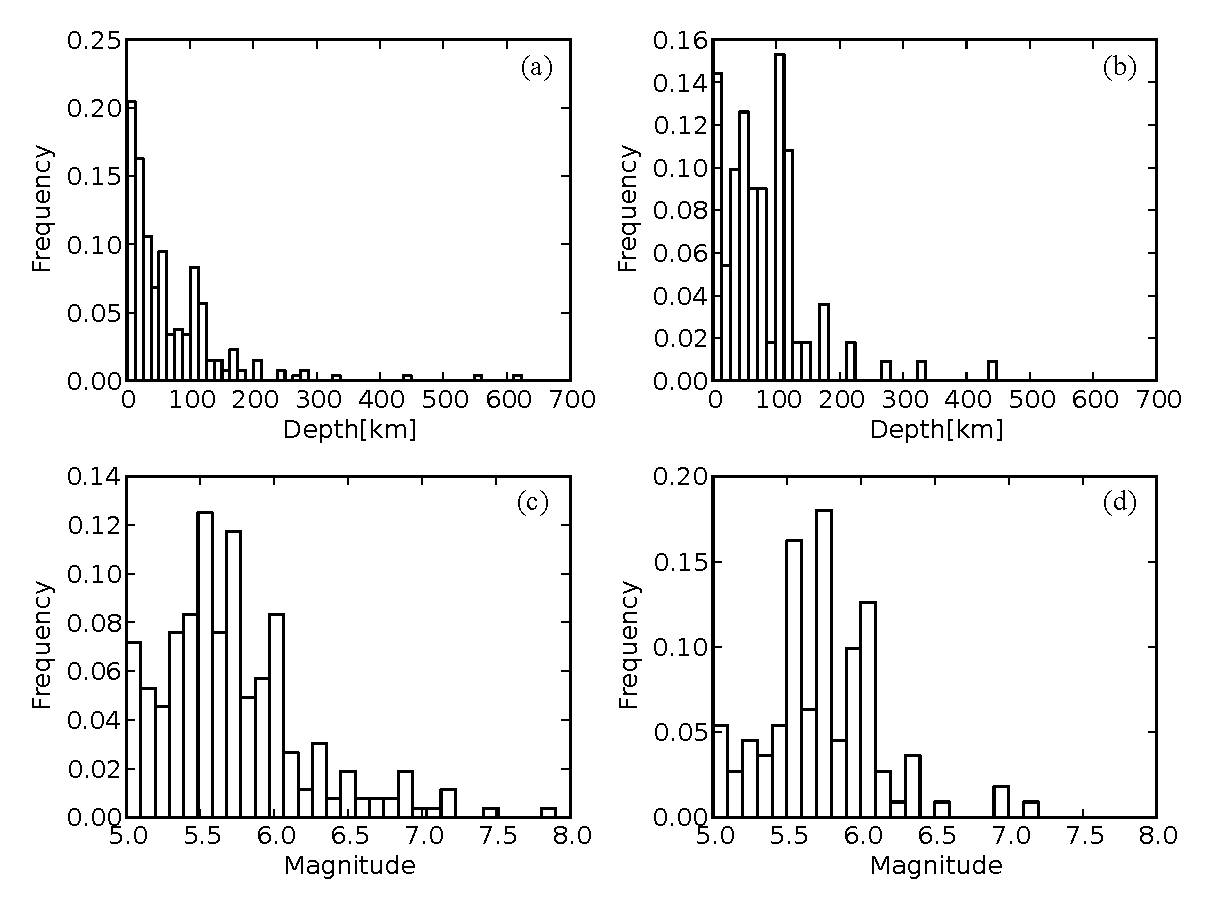
\includegraphics[width=0.85\linewidth]{fig/chap4/depmag_hist1.eps}
	\caption{(a)、(b)分别为观测到PKiKP震相的事件和同时观测到PcP和PKiKP的事件随震源深度%
的分布;(c)、(d)分别为观测到PKiKP震相的事件和同时观测到PcP和PKiKP的事件随震级的分布. }
	\label{dep_mag_hist}
\end{figure}

\begin{figure}
	\centering
	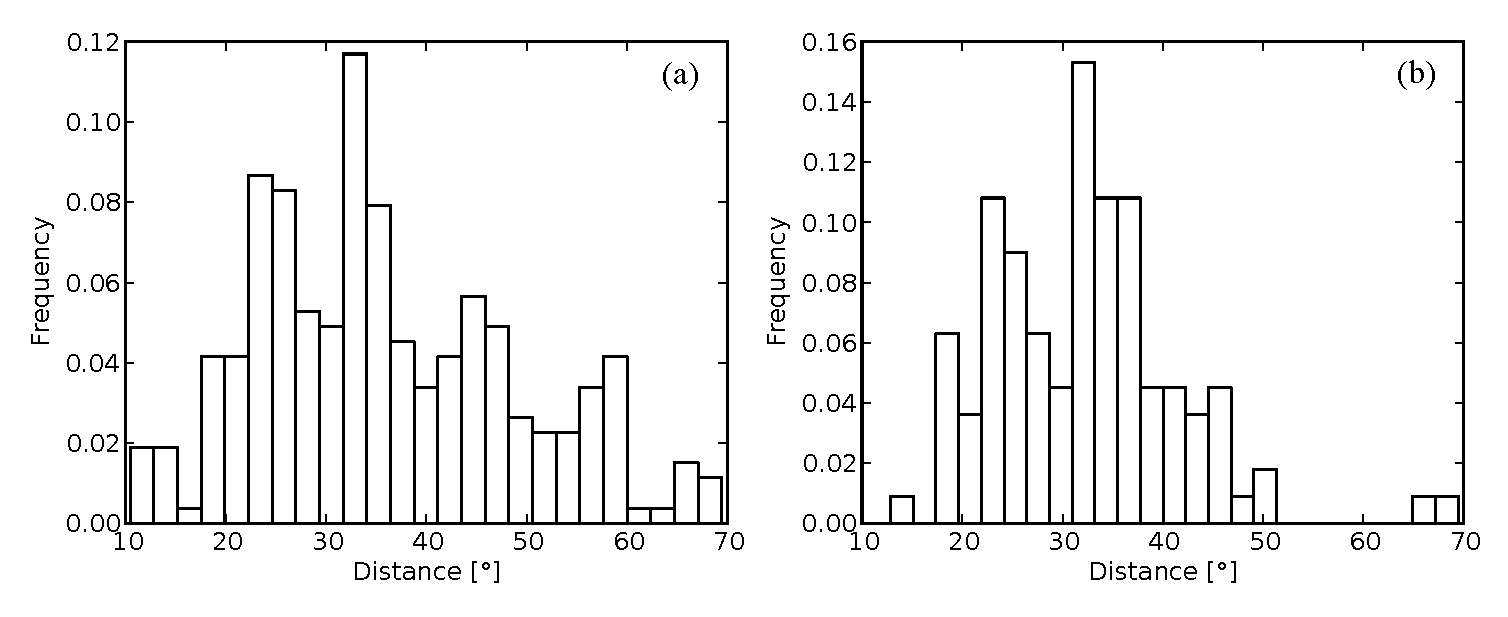
\includegraphics[width=0.85\linewidth]{fig/chap4/dist_hist1.eps}
	\caption{(a)、(b)分别为观测到PKiKP震相的事件和同时观测到PcP和PKiKP的事件随震中距%
的分布. }
	\label{dis_hist}
\end{figure}

\begin{figure}
	\centering
	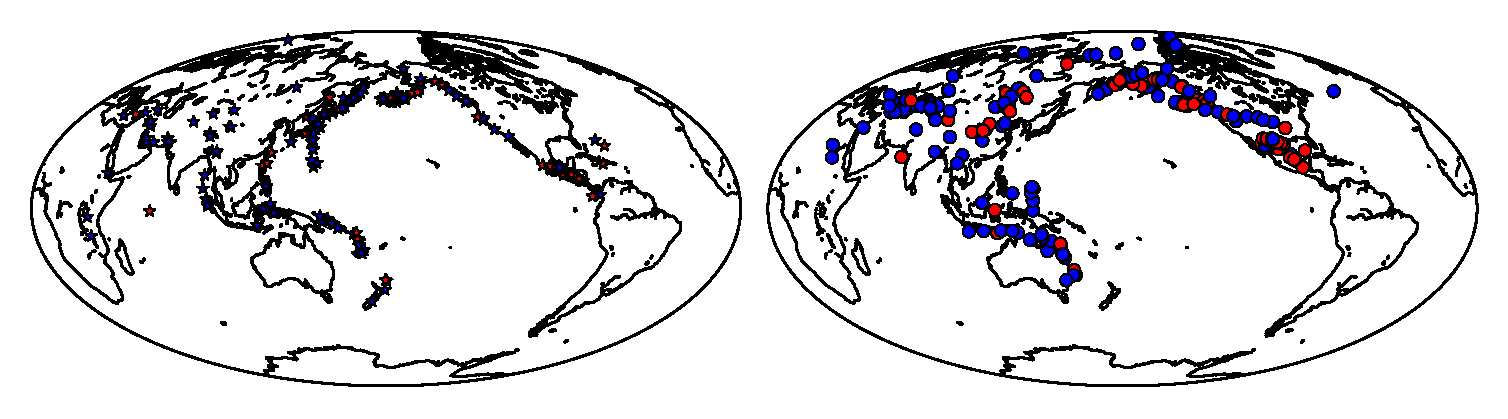
\includegraphics[width=\linewidth]{fig/chap4/loc_distri.eps}
	\caption{左图为地震事件的分布,红色五角星表示同时观测到PKiKP和PcP的事件,蓝色五角星表示%
仅观测到PKiKP的事件;右图为PcP在CMB的上的反射点分布,红色圆圈表示同时观测到PKiKP和PcP,蓝色%
圆圈表示仅观测到PKiKP的反射点. 红色与蓝色的交替体暗示CMB存在小尺度结构的变化. }
	\label{loc_distri}
\end{figure}

\section{CMB界面起伏}

CMB的界面起伏包括其上凸和下陷,分别会造成PcP的发散和汇聚,从而减小或增大台站记录到的PcP振幅~\citep{Neuberg1991}. 本小结基于采样相邻CMB和ICB区域的PKiKP与PcP的振幅比的差异,并结合相对PREM的差异走时残差分析CMB的小尺度起伏变化. 由于本研究主要考虑确定对PcP产生影响的CMB变化因素,因此重点关注的是相邻采样点的振幅比和走时残差的差异,并不要求根据绝对值来约束CMB变化的细节,因此不对所有的观测数据作过多解释. 

\subsection{CMB的局部上凸}

 前人利用全球PKiKP和PcP数据研究ICB物性参数的研究都曾报道过某些区域存在较大的振幅比值,例如\citet{Koper2004a}观测到Vanuatu俯冲带的地震产生的接近理论PREM预测十倍的观测振幅比,并将其解释为CMB起伏和波速异常的综合效应;\citet{Waszek2015a}则将很多大的振幅比观测归结于ICB对PKiKP的放大. 本研究
中采样中美洲下方的CMB的NVAR和PDAR数据很大程度上可以用一个局部上凸的CMB来解释. 对于表\ref{evt}
中前10个地震事件,它们产生的PcP和PKiKP同时被NVAR与PDAR记录到,本研究通过比较与CMB上不同的PcP反
射点位置所对应的PKiKP/PcP振幅比,发现了对于不同反射区域,振幅比存在非常明显的差异. 这10个地震按照地
理位置关系大致可以被划分为两组. 纬度较高的一组包含3个地震,位于墨西哥南部;而纬度较低的一组包含7个地
震,位于危地马拉地震带(图\ref{map}a). 位于下方的一组中的地震的震源机制相似正断型的震源机制,但深
度都不相同,从数十至一百km左右. 

\begin{figure}
\centering
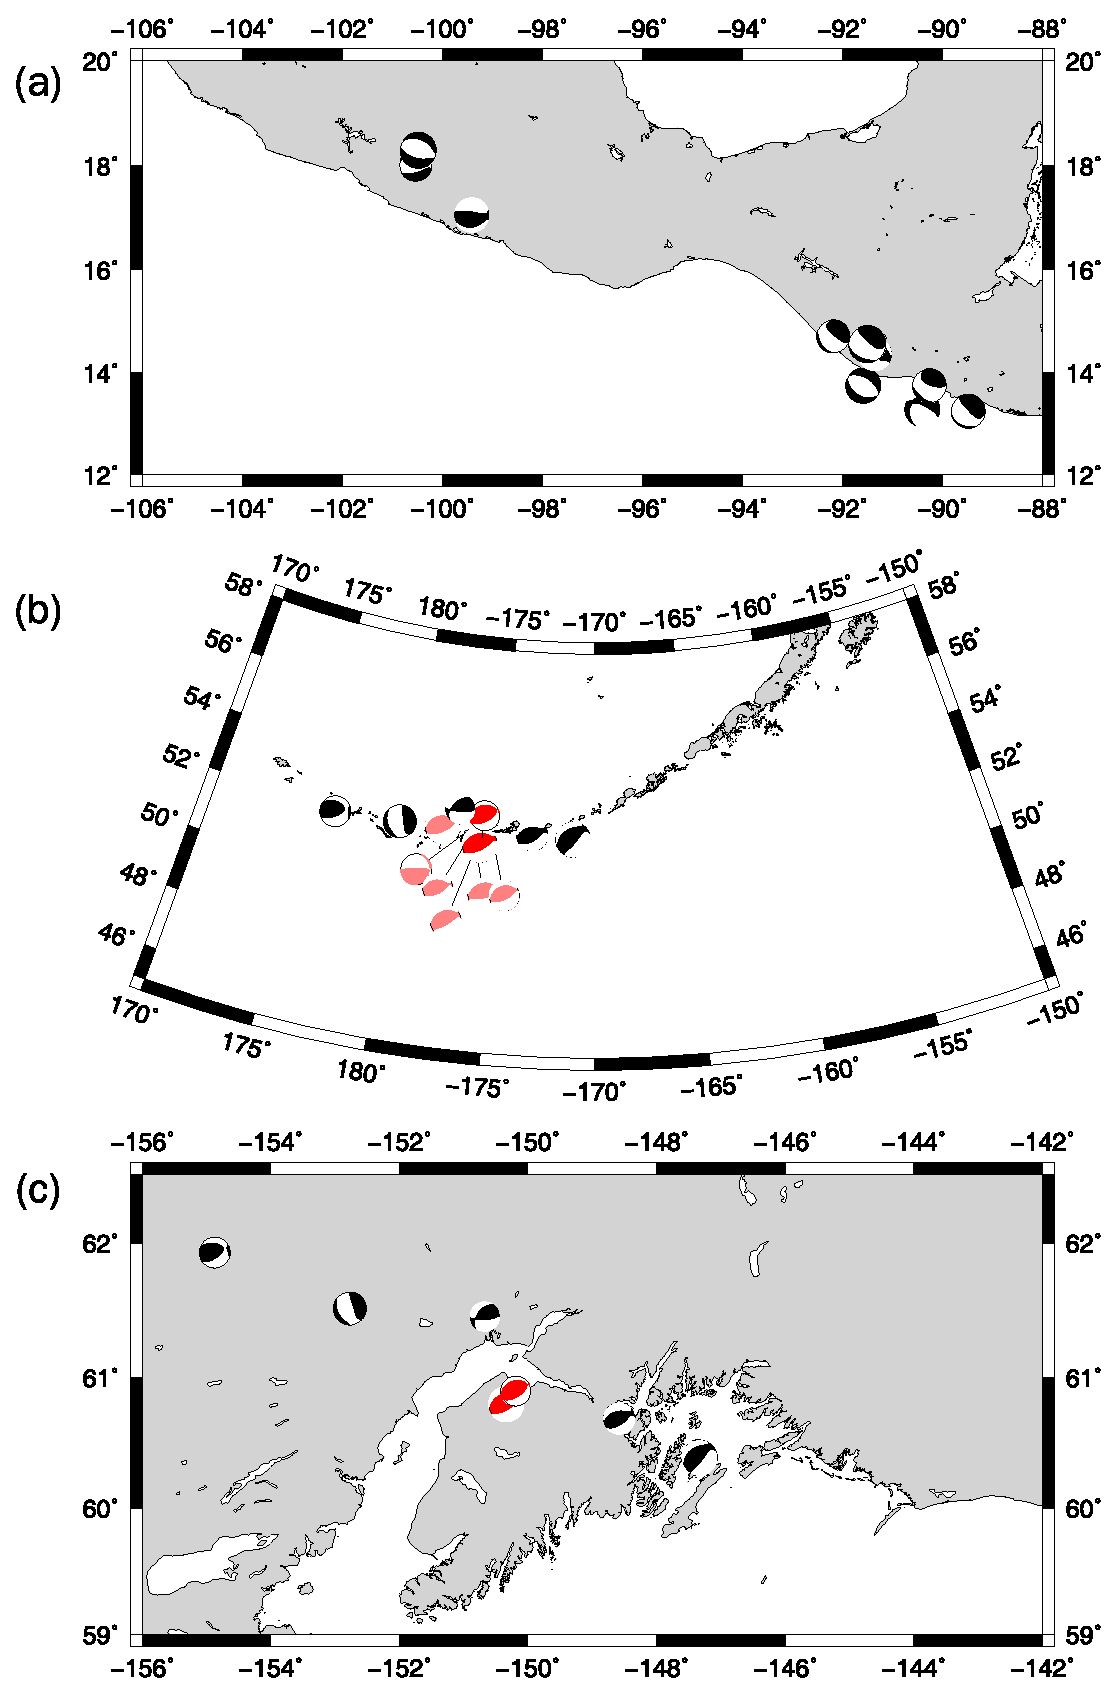
\includegraphics[width=0.7\linewidth]{fig/chap3/evt_bp.eps}
\caption{(a)~表\ref{evt}中第1--10号地震的位置;(b)~黑色和红色的震源球表示是表\ref{evt}中第11--17号地震, 红色震源球表示产生相对与相邻地震异常小的振幅比的事件. 浅红色的震源球表示地震产生与小振幅比事件相似的大振幅PcP,但没有PKiKP的观测;(c)~(b)中黑色和红色事件产生的PcP在CMB上的反射点位置. }
\label{map}
\end{figure}

根据这十个地震-台阵对的PcP反射点的位置,可以在CMB上划分出四个小反射区域,如图\ref{ratio_loc}所
示. 通过测量每个事件-台阵平均PKiKP/PcP振幅比,可以注意到对应于位于危地马拉的7个地震,NVAR和PDAR
记录到的振幅比的明显差异(图\ref{ratio_loc}b),这也体现出相应的CMB上的PcP反射区域1和4的性质存
在明显的差异. 对于NVAR,其观测振幅比相比于由PDAR记录的振幅比要小很多,然而这两个台阵的震中距比较接近,仅相差1{\textdegree}左右,因此可以排除震中距差异的影响. 对于下方7个地震的振幅比测量,NVAR的结果
几乎都是0.03左右,且平均振幅比的标准差全小于0.008,仅有事件7稍大为0.067,与PREM对各项同性源的预测
值0.04还是比较接近的. 这也体现出对于这些地震,NVAR的振幅比测量结果是比较稳定和可信的. 与NVAR台阵的测
量结果相反,使用PDAR的记录得到的PKiKP/PcP振幅比则普遍偏大,均为PREM理论值的两倍以上,同时也具有很
大的标准差. 关于标准差的差异,可以解释为,当PcP振幅很大且变化不大的情况下,由于其位于分母且PKiKP振幅
都比较小,造成最终的振幅比偏小且每道的值相差不大,这就对应NVAR的结果;而PcP振幅较小,若其稍有变化,
便使得振幅比有较大的变化,这就对应PDAR的情况. 以上分析也表明,PDAR记录到的PcP受到了强烈的衰减. 对于
上方3个地震,NVAR和PDAR的观测振幅还较为接近,均为PREM预测的数倍. 

进一步比较采样区域1和4的数据,可以推断出CMB结构对振幅比的强烈变化有重要贡献. 首先,从振幅的角度看,与
相对稳定PKiKP相比,两个位置反射的PcP振幅显示出了很大的差异. 对于事件10,在观测的频率范围(1--2 Hz) ,NVAR和PDAR记录的PcP振幅大小明显不同,NVAR的PcP叠加振幅要比PDAR的要大6倍以上,然而,两个台阵的叠加PKiKP振幅却十分相近(图\ref{amp_nv_pd});其次,从波形的角度来看,采样两个区域的PcP波形也存在显著差异(图\ref{amp_nv_pd},\ref{pcp_pkikp_nvpd}). 采样区域1的PcP波形显得相对尖锐,而采样区域4的PcP显得波形被延长了;与PcP的差异产生鲜明对比的是,两个台阵记录的PKiKP波形都显得清晰尖锐. 除此之外,由NVAR记录的PcP波形与两台阵记录的PKiKP波形也比较相似. 不仅对事件10,出现这种现象,对于图\ref{map}中下方其他几个地震也是如此. 这就有力地表明,造成PcP波形和振幅的变化的源头并非来自浅部的衰减或不均匀结构,因为在浅部PKiKP和PcP具有相近的传播路径,因而会有相似的特点. 所以可以把造成PcP和PKiKP/PcP振幅比差异的源头继续追踪至CMB的结构. NVAR和PDAR间距约为1000km,而1和4两个反射区域在CMB上距离约为280km,这可能暗示了CMB在中等尺度下的变化. 

\begin{figure}
\centering
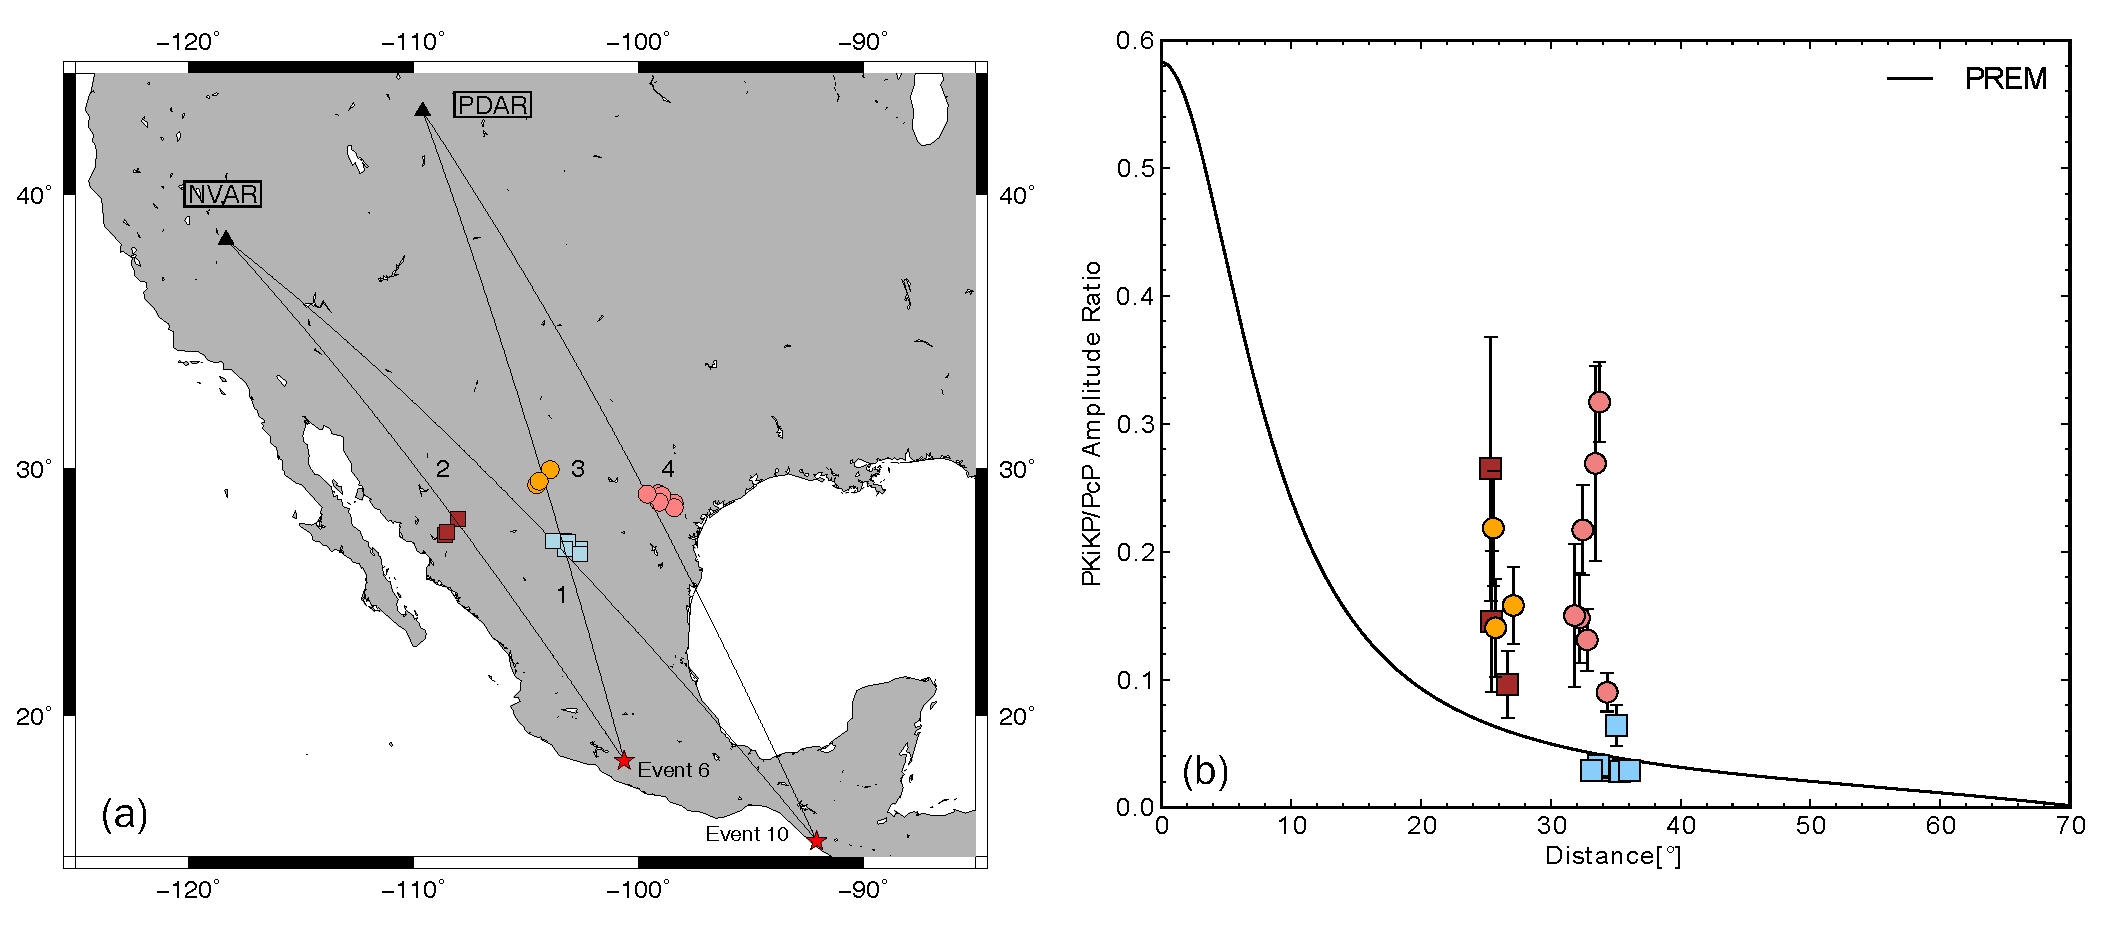
\includegraphics[width=\linewidth]{fig/chap3/evt_bp_us.eps}
\caption{(a)~台阵NVAR、PDAR和表\ref{evt}中前十个事件的PcP反射点位置. 两个台阵和事件6、10的位置也被画出. 浅蓝色圆圈表示相应与较低PKiKP/PcP振幅比的PcP反射点位置,浅红色圆圈则表示相对大的振幅比. 四个PcP反射区域用数字1--4标出;(b)~NVAR和PDAR观测到的由图\ref{map}下方事件组产生的PKiKP与PcP信号的振幅比. 可以看出两个台阵观测的明显差异. PREM对与一个各项同性源的预测振幅比值也被画出,作为参考. }
\label{ratio_loc}
\end{figure}

\begin{figure}
\centering
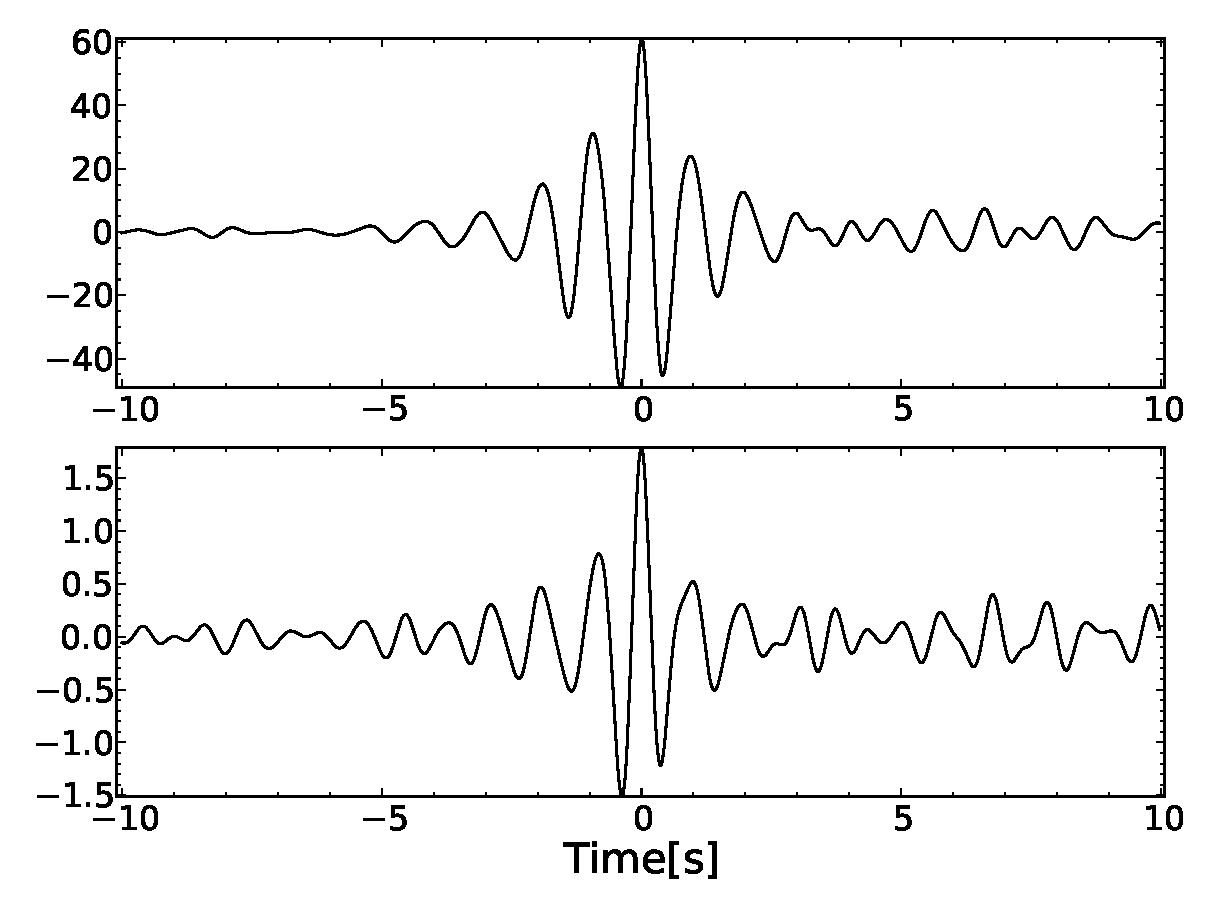
\includegraphics[width=0.4\linewidth]{fig/chap3/amp_nv_4371355_s.eps}
\quad
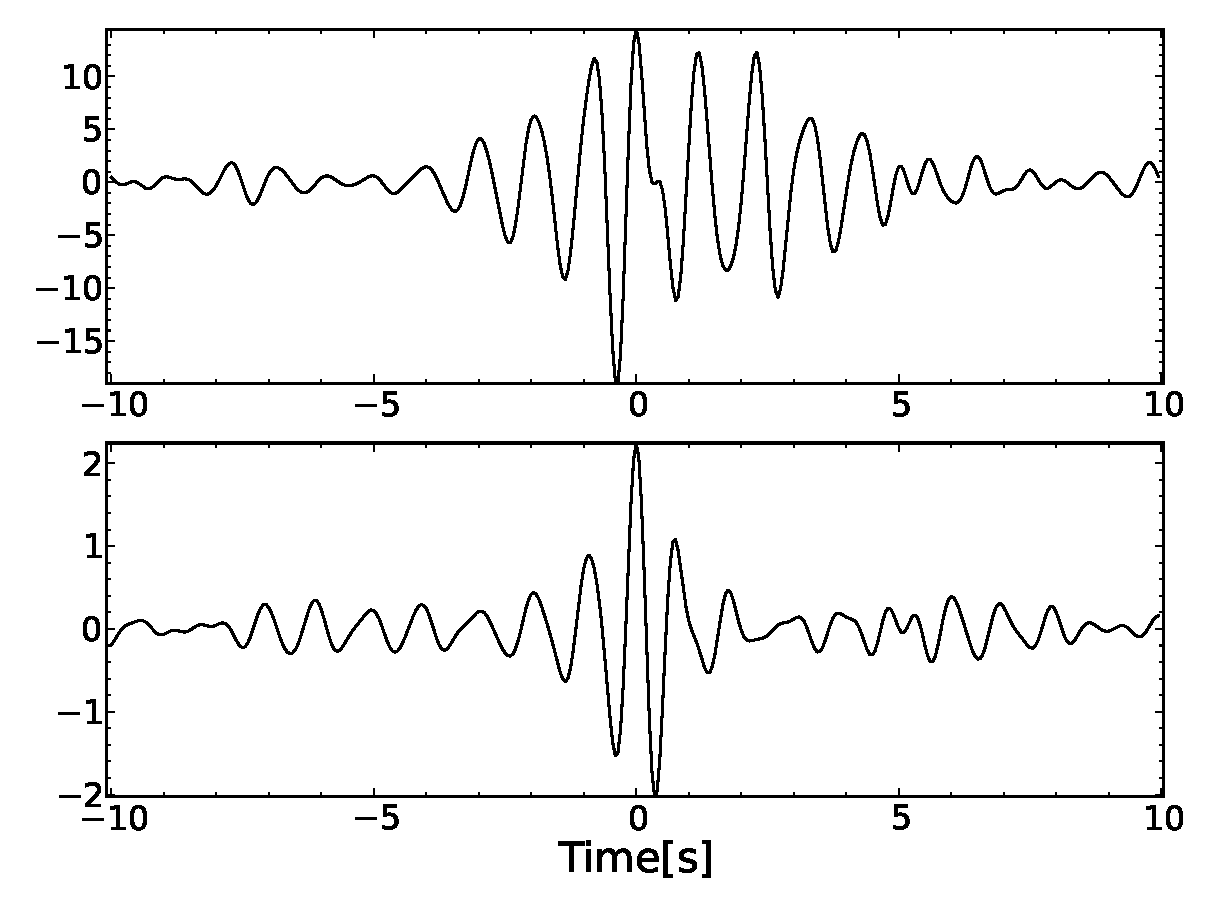
\includegraphics[width=0.4\linewidth]{fig/chap3/amp_pd_4371355_s.eps}
\caption{表\ref{evt}中事件10产生的PcP and PKiKP,分别由(a)~NVAR和(b)~PDAR所记录. 波形均为台阵内所有台站的叠加,震中距标在图的左上角. }
\label{amp_nv_pd}
\end{figure}

\begin{figure}
\centering
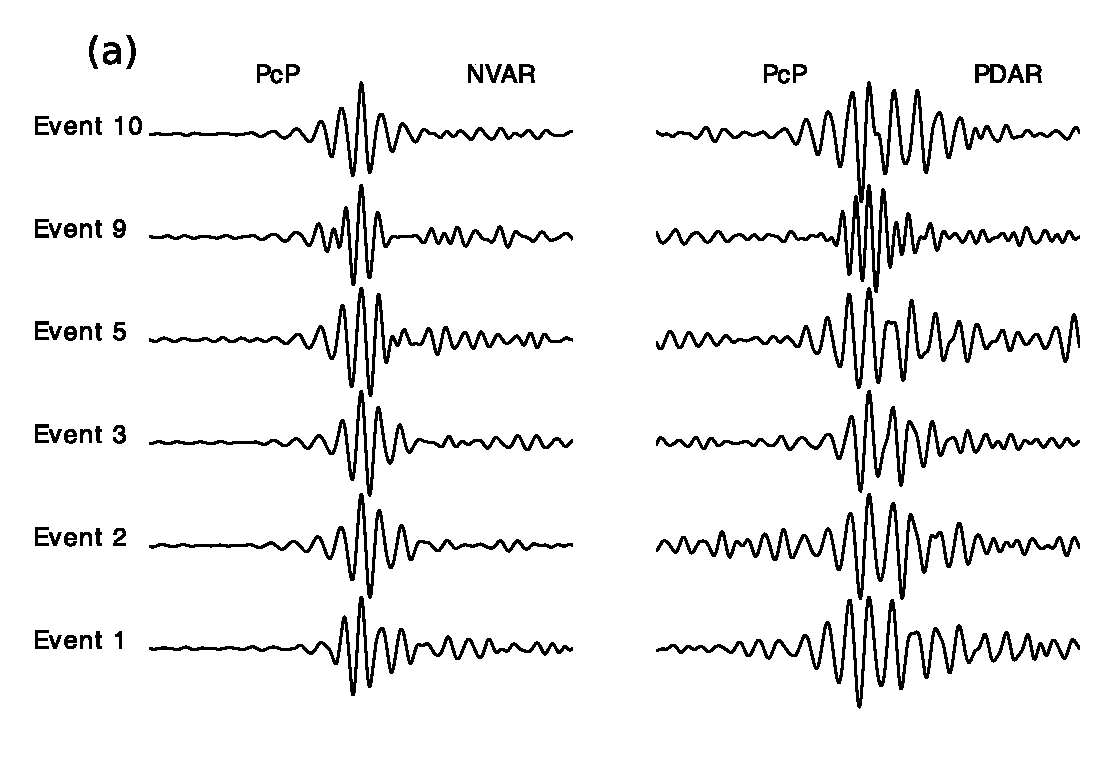
\includegraphics[width=0.7\linewidth]{fig/chap3/pcp_nvpd.eps}
\\
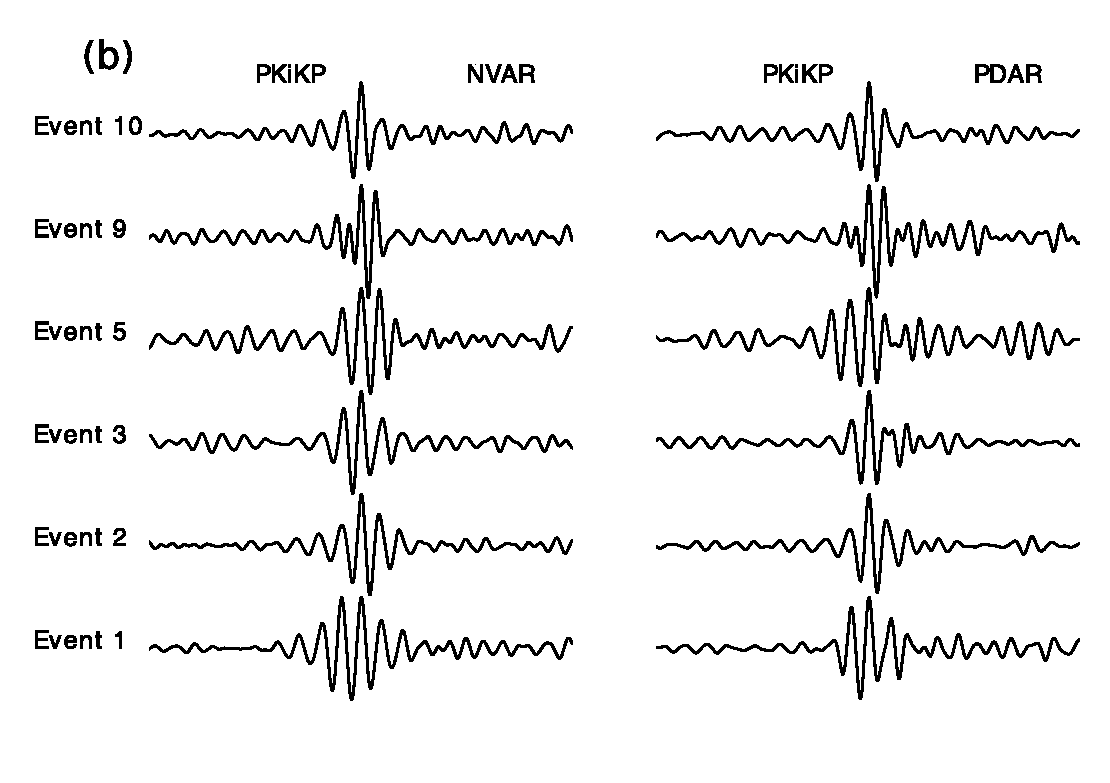
\includegraphics[width=0.7\linewidth]{fig/chap3/pkikp_nvpd.eps}
\caption{NVAR和PDAR记录的表\ref{evt}中6个事件的PcP(a)和PKiKP(b)波形比较. 采样区域1和区域4的PcP波形有显著不同,而PKiKP则具有相似的特点. 图中所有记录均为台阵的叠加波形. }
\label{pcp_pkikp_nvpd}
\end{figure}

接下来再将以上的观测结果与最近关于起伏CMB下的PcP模拟结果比较\citep{Wu2014a},可以发现两者具
有很好的一致性. 根据模拟结果,一个局部上凸的CMB可以造成PcP振幅的减小同时伴有波形的延长,而这正是
本研究所观测到的现象. 还可以注意到,对于事件9,PDAR记录的PcP波形和PKiKP相比并没有太大变化,而且平
均台阵PKiKP/PcP振幅比为0.09,这可能意味着对于这个事件-台阵对,PcP受到了较小的界面起伏的影响. 为了
进一步验证上面的观测,再对采样区域4的USArray数据进行检查,这里选取距离PDAR为2{\textdegree}以内
的USArray台站的数据,结果也显示,在存在较清晰PKiKP波形的情况下,PcP的波形也和PDAR台阵的记录一致,
这也很大程度排除了台站因素对观测的影响. 

由于这两个台震数据采样的区域位于俯冲带的下方,因而CMB的隆升可能与古俯冲板块的残片在CMB堆积有某种联系. 

\subsection{CMB的局部下陷}

除了CMB的上凸,CMB的局部下陷的情况也同样存在. \citet{Rost2004a}曾报道了在阿拉斯加Kenai半岛
下方的CMB上存在这样一个凹陷,造成PcP振幅的异常放大. 该研究发现在Kenai半岛下方采样的PcP与P波的
振幅比远高于理论估计值,由此推断此处的CMB很可能存在一个下凹. 但影响PcP/P振幅比的因素还有很多,
比如(1)P波传播路径的高衰减;(2)俯冲板块的聚散焦效应;(3)CMB上方的波速、密度异常,或者CMB的界面起伏
. 之前的研究通过分析各种情形下,PcP/P振幅比的变化,最终认为CMB起伏是最可能的异常来源. 然而,将P作为
参考震相,来约束CMB结构,其引入的很多不确定性还是不能被消除,毕竟P和PcP在上地幔中的传播路径还是有很
大差异,因此它们经历不同的衰减和不均匀结构的可能性还是很大. 考虑到各种因素,估计的CMB起伏对PcP的放大
效应就可能并不明显. 

为了尽量避开上面的问题,本研究使用PcP和PKiKP组合来进一步验证之前研究所提出的Kenai半岛下方CMB下凹的
情形. 图\ref{map}b中的7个地震均产生了能被YKA台阵记录到的PcP和PKiKP,其中事件14和15的记录显示
出约为PREM预测二分之一的PKiKP/PcP振幅比,PcP的反射点位置几乎和之前研究发现的高PcP/P振幅比的区域
一致(图\ref{map}c),除此之外,在这两个地震发生位置很近的地方,有很多产生相似大振幅PcP的地震,但
没有观测到相应的PKiKP. 与这两个地震不同,其余5个地震均没有产生这样低的振幅比,特别是与这两个地震相邻
的另外两个地震. 如果假设,在很小的范围内,ICB并无太大变化,则可能是Kenai半岛下方CMB上的某种变化使得
PcP的振幅被放大了. 由于研究用到的7个地震均沿着阿留申群岛分布,它们产生的PcP反射点在CMB上大致形
成一条长约500km的线状剖面,这样就可以使得细致地研究该区域的CMB界面起伏提供了可能. 

\begin{figure}
\centering
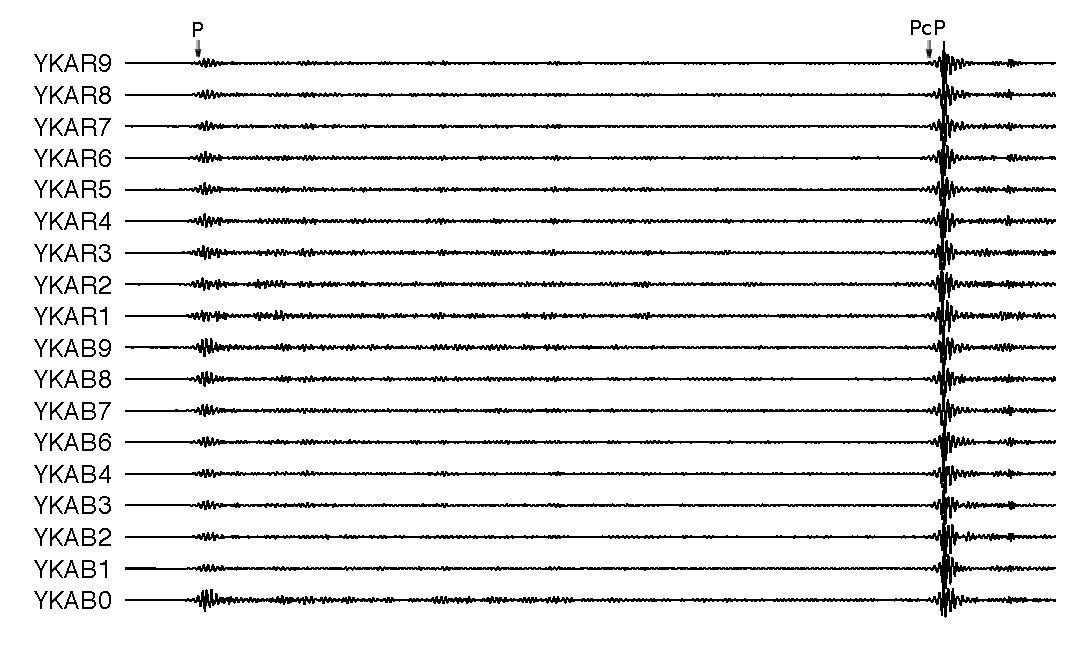
\includegraphics[width=0.87\linewidth]{fig/chap3/p_pcp_4599655.eps}
\caption{YKA对事件2014/04/21 14:02:15(Mw 
5.4, 54 km)产生的P和PcP记录. 每一道按照PcP振幅归一化, 可以明显看出台站间P波的振幅差异. }
\label{p_pcp}
\end{figure}

通过观察事件14、15每道记录的P和PcP振幅,可以发现即使在同一台阵内,台站间的P波振幅差异可以达到2倍,而PcP的振幅差异则很小,因此若将每道记录的振幅按照PcP振幅归一化,可以明显看出P波振幅的变化(图\ref{p_pcp}). YKA台阵位于稳定的克拉通岩石圈之上,其所处区域经受了稳定的沉积过程,所以这可能是由于台阵下方存在的沉积结构对P波的衰减,而PcP由于其相对小的慢度,受到的影响较小. 仅考虑这一点,使用P作为参考将为就会造成对CMB结构不正确的估计,以此使用PKiKP作为参考相就显得很有必要. 

\begin{figure}
\centering
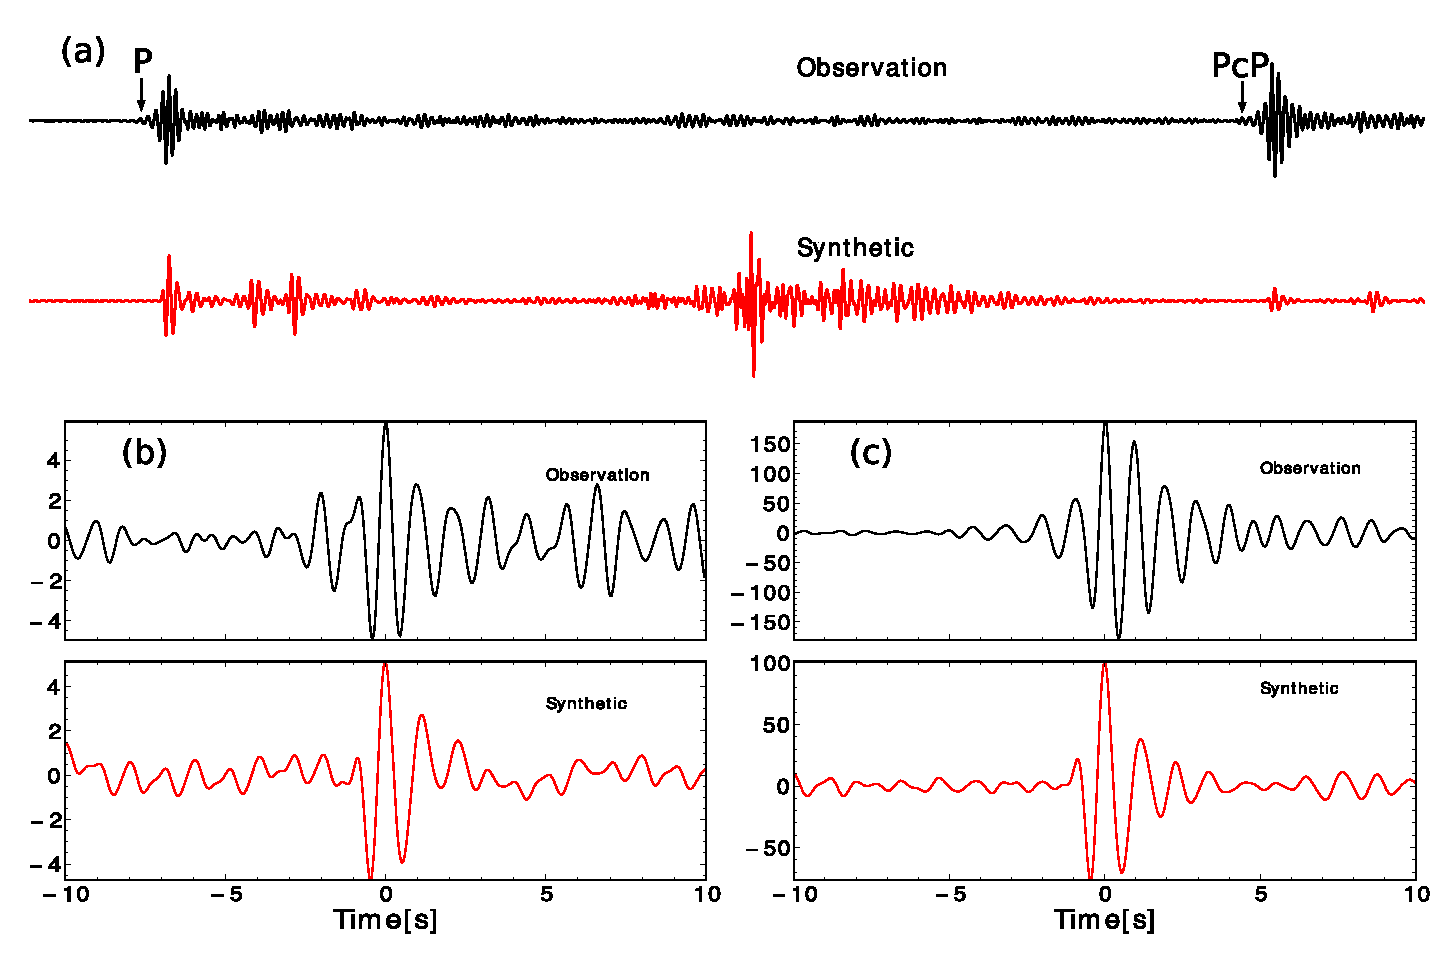
\includegraphics[width=0.85\linewidth]{fig/chap3/syn_2}
\caption{YKA台阵对表\ref{evt}地震14的记录和DSM理论地震图. (a)观测和理论的P和PcP的振幅比较;(b)观测和理论的PKiKP振幅比较;(c)观测和理论的PcP振幅比较. 其中观测记录来自台站YKB8. }
\label{fig:syn_2}
\end{figure}

\begin{figure}
\centering
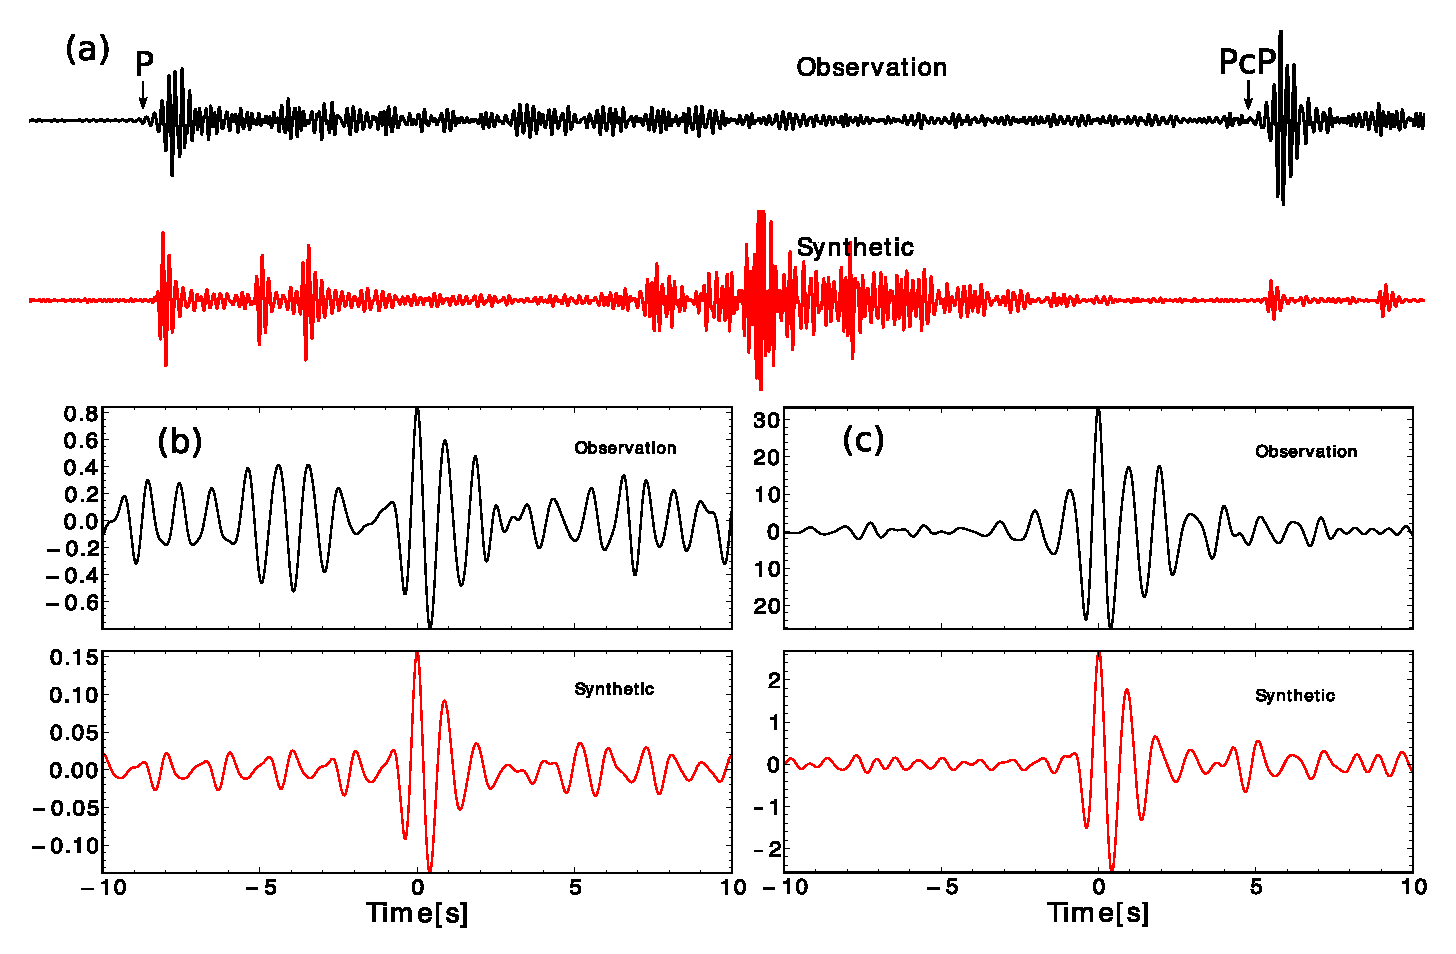
\includegraphics[width=0.85\linewidth]{fig/chap3/syn_3}
\caption{YKA台阵对表\ref{evt}地震15的记录和DSM理论地震图. (a)观测和理论的P和PcP的振幅比较;(b)观测和理论的PKiKP振幅比较;(c)观测和理论的PcP振幅比较. 其中观测记录来自台站YKAR9. }
\label{fig:syn_3}
\end{figure}

\begin{figure}
\centering
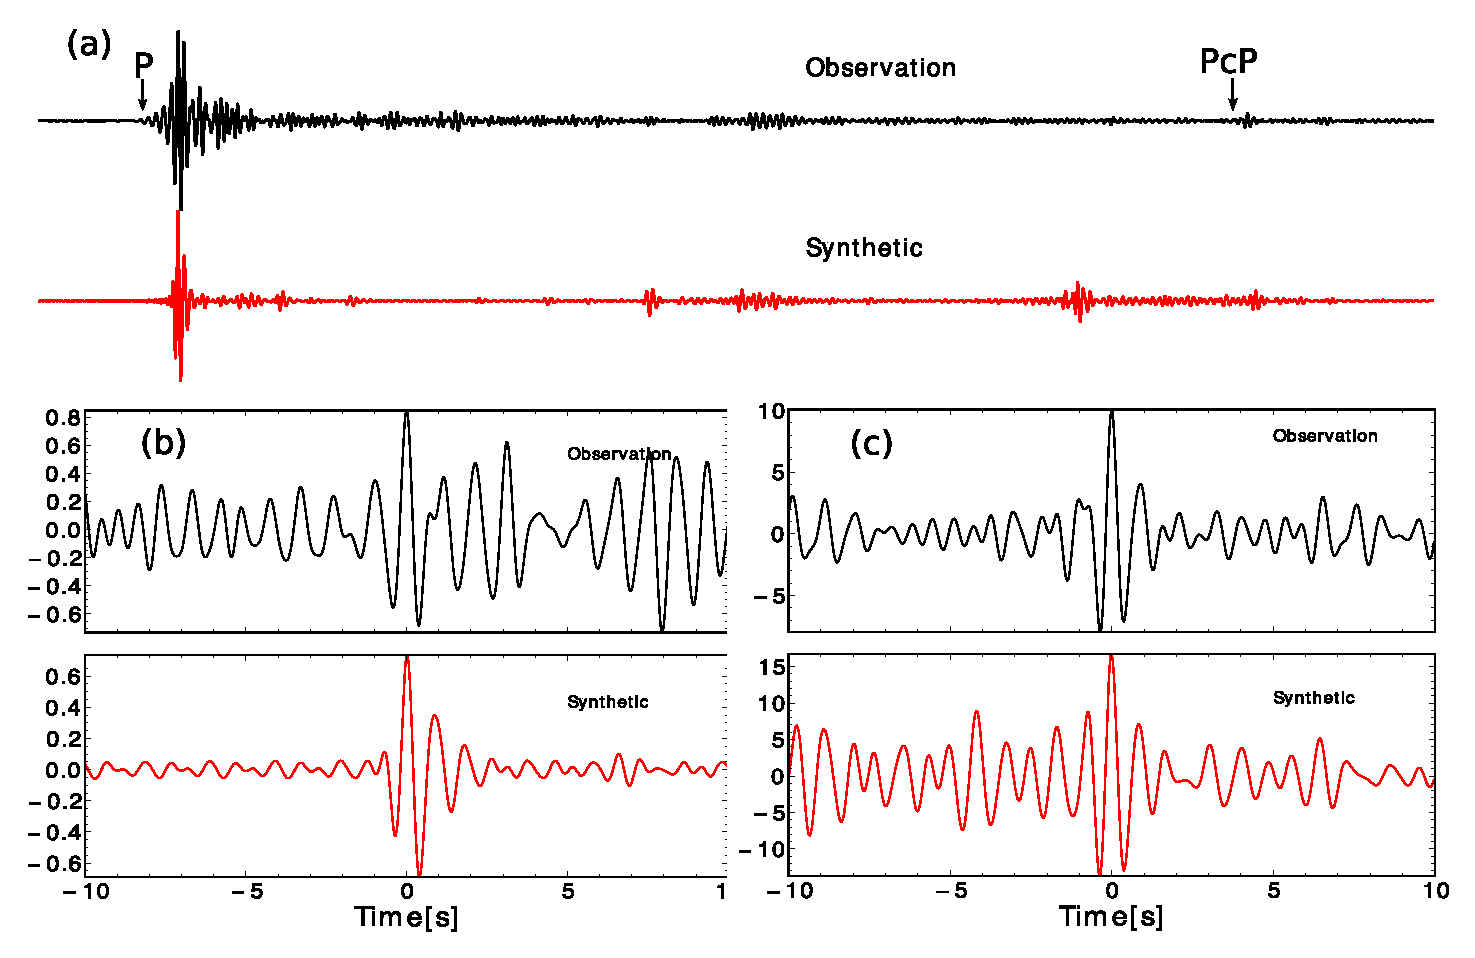
\includegraphics[width=0.85\linewidth]{fig/chap3/syn_1}
\caption{YKA台阵对表\ref{evt}地震13的记录和DSM理论地震图. (a)观测和理论的P和PcP的振幅比较;(b)观测和理论的PKiKP振幅比较;(c)观测和理论的PcP振幅比较. 其中观测记录来自台站YKAR9. }
\label{fig:syn_1}
\end{figure}

\begin{figure}
\centering
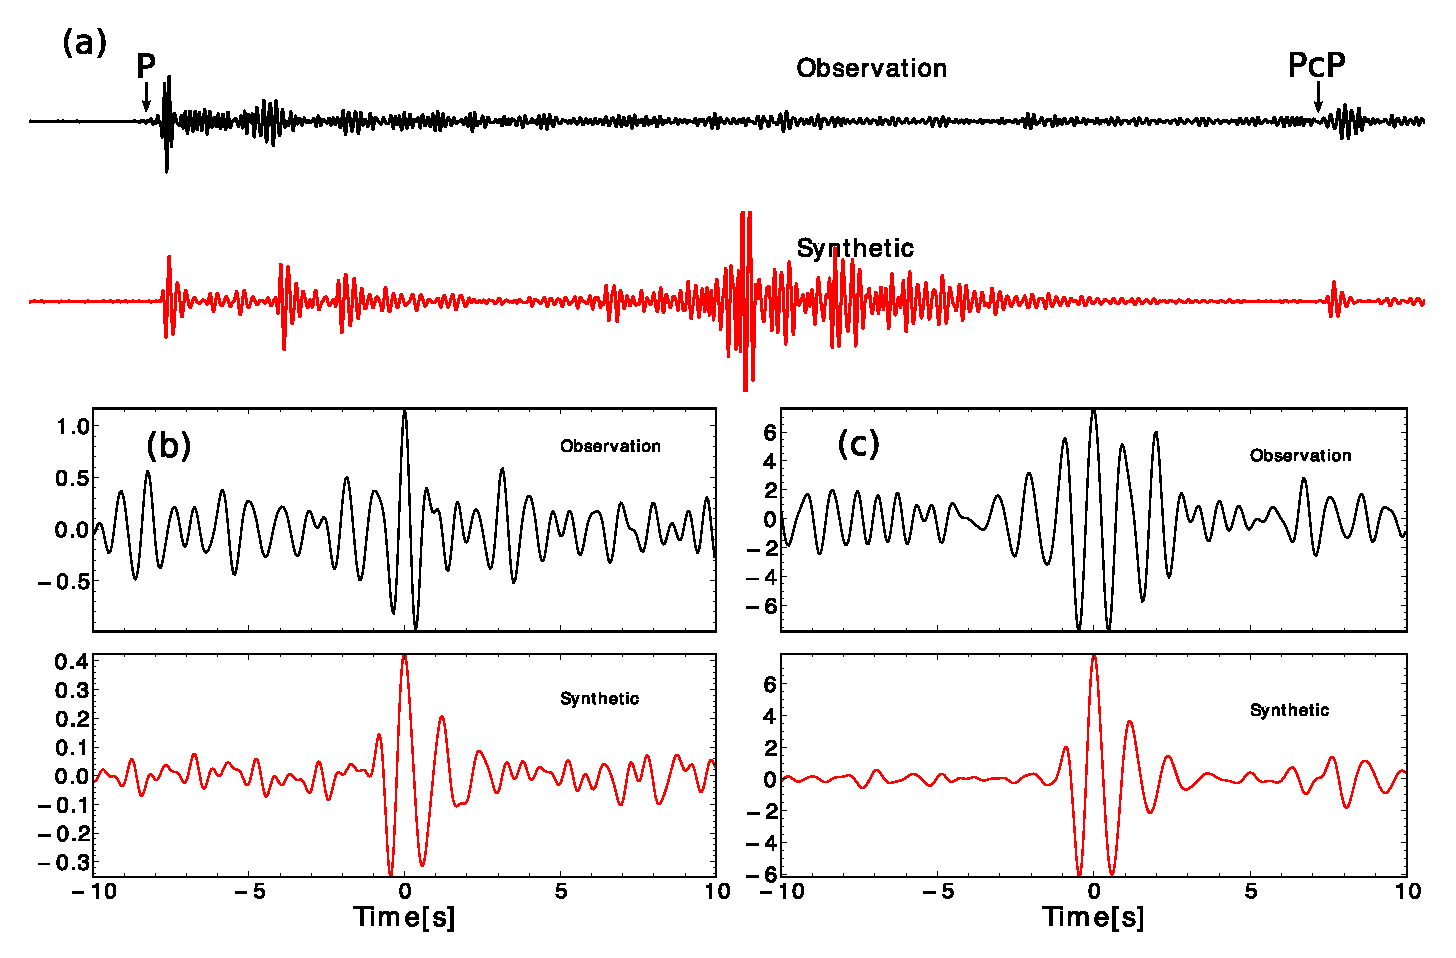
\includegraphics[width=0.85\linewidth]{fig/chap3/syn_4}
\caption{YKA台阵对表\ref{evt}地震16的记录和DSM理论地震图. (a)观测和理论的P和PcP的振幅比较;(b)观测和理论的PKiKP振幅比较;(c)观测和理论的PcP振幅比较. 其中观测记录来自台站YKR2. }
\label{fig:syn_4}
\end{figure}

为了消除震源对P、PcP和PKiKP振幅的影响,这里再使用DSM~\citep{Takeuchi1996,Kawai2006}计算理论地震图,将其与观测记录比较,进一步对PcP被放大的推测作检验. 为了尽量减小P波受台阵下方结构衰减对分析的干扰,所用的观测记录均选取台阵内具有最大P波振幅的台站记录. 可以发现,对于两个产生异常小振幅比的事件,DSM计算的PcP振幅比P波振幅小,与观测记录有很大差异,PKiKP/PcP振幅比也比DSM预计的要小一倍(图\ref{fig:syn_2},\ref{fig:syn_3});而对于
另外两个相邻地震,观测的的P/PcP振幅比并没有明显小于DMS预测的振幅比,反而PKiKP/PcP振幅比却比预测值
要大(图\ref{fig:syn_1},\ref{fig:syn_1}). 通过测量这七个事件的PKiKP-PcP相对PREM的差异走时
残差,也发现残差也恰好可以与一个Kenai半岛下方下凹的CMB对应(图\ref{fig:topo}b、c). 还
可以注意到,这7个地震的PKiKP/PcP振幅比和PKiKP-PcP差异走时残差之间存在一个正相关,这表明振幅比可能
与CMB或者ICB的起伏变化有所联系,而本研究更加倾向于前者,因为根据观测,PcP的变化要比PKiKP更加显著. 
观测到的Kenai半岛下方达到1.5秒的负走时残差也和之前的研究一致~\citep{Koper2004a,Waszek2015a},进一步验证了该区域走时残差测量的可靠性. 

在CMB处1$\sim$2Hz的PcP菲涅尔半径约为120km~\citep{Tkalcic2009},并且当CMB起伏的横向尺度和PcP的菲
涅尔带相当的时候,CMB起伏才会对PcP的振幅造成显著的影响~\citep{Wu2014a},因而图\ref{fig:topo}c中所描述的起伏尺度似乎也是比较合理的. 从7个地震的PcP-PKiKP差异走时残差的相对变化来看,观测值与标准模
型之间存在一个系统性的偏差,这可能是该区域下方的外核厚度有整体的变薄. 总而言之,所有的观测都支持该区域CMB存在一个局部下凹,但由于ICB的起伏变化仍然是未知的,而且走时残差仍然受地幔结构的影响,因此得到准确的界面起伏尺度仍然存在困难.

\begin{figure}
\centering
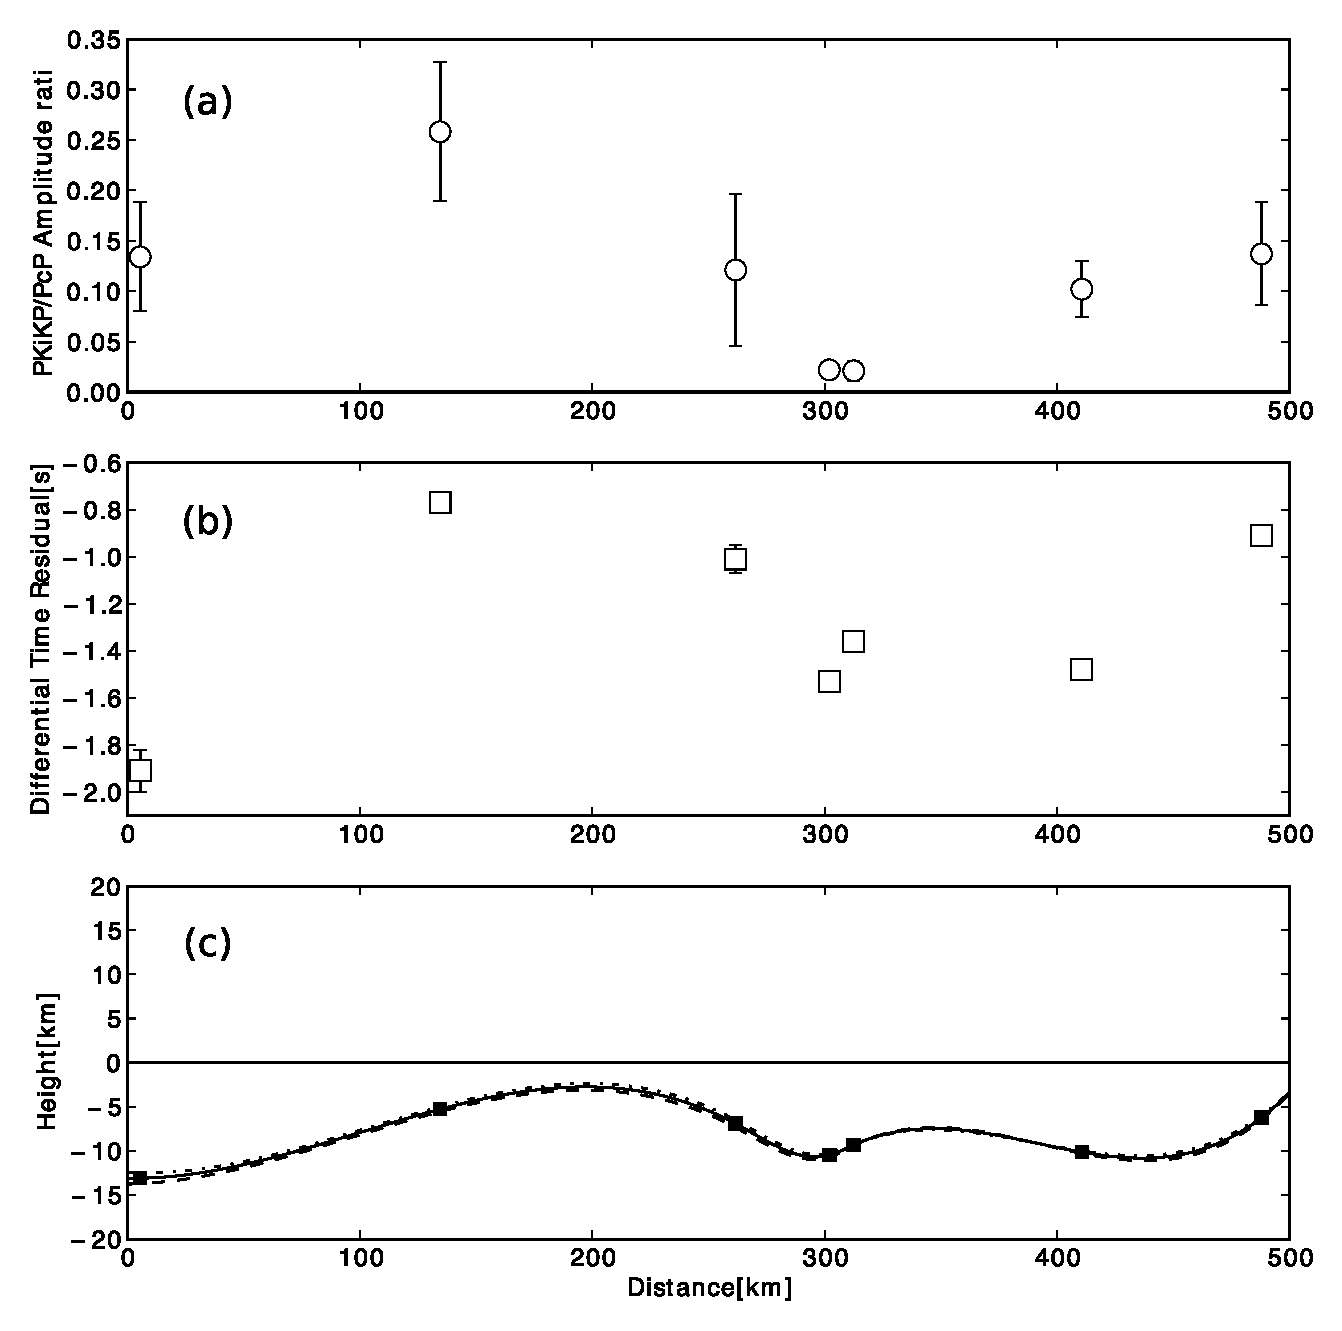
\includegraphics[width=0.7\linewidth]{fig/chap3/topo}
\caption{(a)YKA记录的图\ref{map}b中7个地震的PKiKP/PcP平均振幅比;(b)对应图\ref{map}c中反射点的PKiKP-PcP差异走时残差;(c)利用关系$H=\frac{t}{\sqrt{\frac{1}{V^2-p^2}}}$,可以将走时残差转换为深度变化,然后在插值得到界面的起伏变化. 点线和虚线表示应台阵走时残差的标准差. }
\label{fig:topo}
\end{figure}

由上面的观测,可以认识到CMB的起伏可能会出现比较复杂的情况,而产生这些复杂变化的则是复杂的外核和地幔的动力学过程. \citet{Lassak2010a}通过地球动力学模拟,认为地幔底部的物质堆积(Pile)和地幔柱在CMB起伏变化的形成过程中起到了重要作用. CMB上的物质堆积或地幔柱的上升流下方均对应CMB的隆升,而与俯冲板块相联系的下降流下方的CMB则呈现出凹陷. 但通过模拟难以将这两类模型的效应区分开,本研究所探测到的CMB小尺度界面起伏变化可能有助于缩小用于解释CMB结构变化的模型空间. 同时,形成当前地幔的速度结构和CMB起伏的动力学过程也不是相互独立的,通过地幔对流,它们可能存在相互耦合~\citep{Forte1991a}. 即地幔底部的速度异常和CMB的起伏存在某种对应关系~\citep{Forte1994a},如果将这种关系代入到地震波走时反演中就可以减少反演参数,从而得到更有物理意义的CMB模型~\citep{Soldati2012a}.

\subsection{ICB结构和CMB横向不均匀}

以上给出了两个用PKiKP和PcP分析CMB起伏变化的例子,但还有其他因素也会对振幅比和走时残差的观测造成影响,下面对一些主要的影响因素即ICB的结构和CMB横向不均匀性变化作一些讨论. 

\subsubsection{ICB结构}

对于前面的分析中并没有提及太多ICB效应对PKiKP/PcP振幅比和走时残差的影响,通常来说,其影响主要来自界面起伏变化及横向不均匀性变化. 如果这些变化比较显著的话,ICB的效应就不能忽略. 对于前面阿拉斯加的例子,除
了CMB局部凹陷的解释,观测到的异常小的PKiKP/PcP振幅比和大的负走时残差也可以被解释为一个局部上凸的ICB的效应(图\ref{fig:model}). 这样的一个ICB结构可以同时减小PKiKP走时和其振幅,导致负的走时残差和
小的振幅比. 如果是这种情况,PKiKP应该会出现与如图\ref{pcp_pkikp_nvpd}中PcP相似的波形变化,但实际上这并没有观测到,而且PKiKP在小于其菲涅尔半径的区域产生显著的能量发散也似乎是不可能的;另一方面,如果观测也可解释为ICB上局部速度和密度差的急剧降低,这种变化常被认为是ICB上方的小尺度对流的结果~\citep{Krasnoshchekov2005},但对于阿拉斯加的情况,相邻地震在ICB采样区域非常接近,因此出现这样变化的可能性很小,且PKiKP对这种10km级别的变化也不会太敏感. 对于NVAR和PDAR的数据,观测到的同一地震采样两个区域的ICB的PKiKP高度一致,因而ICB的效应可以忽略. 

\begin{figure}[!ht]
\centering
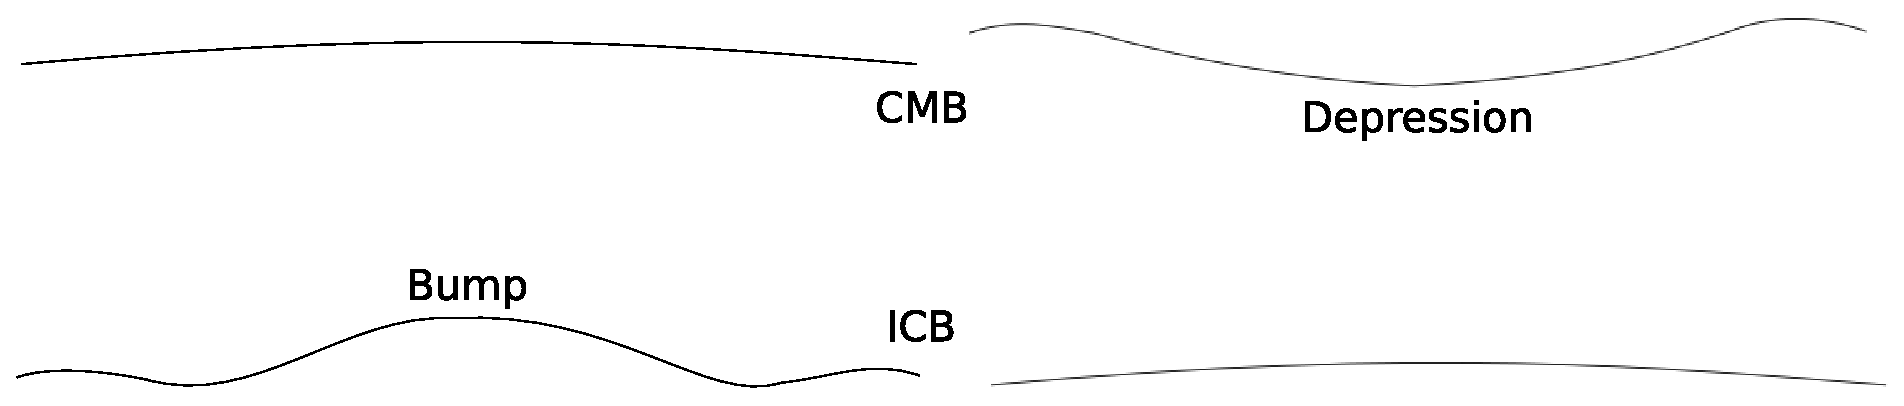
\includegraphics[width=0.7\linewidth]{fig/chap3/model}
\caption{两种可以解释YKA台阵PcP和PKiKP观测的CMB和ICB起伏模式,(左)下凹的CMB和平坦的ICB,(右)平坦的CMB和上凸的ICB. }
\label{fig:model}
\end{figure}

到目前为止,已经有一些研究给出ICB上存在小尺度起伏变化的证据. 其中一些研究使用间接方法,即基于内核差异
旋~\citep{Song1996}造成的ICB随时间变化,利用重复地震对产生的后临界PKiKP的变化来约束ICB起伏~\citep{Wen2006};一些使用前临界PKiKP观测来直接探测ICB起伏变化\citep{Dai2012}. 估计的ICB起伏的高度变化
从数百米~\citep{Cao2007}至数km~\citep{Dai2012},横向尺度也大约也是km的数量级. 对比ICB和CMB起伏的研究,似乎ICB的起伏程度要小于CMB,如果再考虑内外核差异旋转的效应,一个很高的ICB的上凸也是很难维持的. 因此本文认为仅ICB起伏不能完全解释所有的观测. \citet{Krasnoshchekov2005}引入了一种马赛克结构的ICB模型来解释PKiKP的剧烈振幅变化,这种类似补丁的结构由ICB上方薄的部分熔融液体和固体层交替组成,PKiKP在固体或液体层反射后的振幅会有显著不同. 之前的研究认为这种补丁结构是由与内核的不均一冷凝或者是ICB上方的物质对流所致,并估计这种结构的尺度从数十至数百km. 然而,在本研究中,小范围内剧烈的PKiKP振幅变化并没有被观测到,临近区域相同震级的地震产生的PKiKP振幅往往也是接近的,这也说明在本文的研究区域并没有这样的结构存在. 

\subsubsection{CMB横向不均匀性}

除了CMB的界面起伏,其物性的横向的不均匀也会对PcP的产生比较大的影响. 典型的超低速带(ULVZ)通常存在30\%的S波波速和10\%的P波波速的降低~\citep{Thorne2004a},这样的一个低速异常可以有效低降低50\%的PcP反射系数. 然而,仅用ULVZ并不能解释PDAR记录的PcP波形的变化(图\ref{amp_nv_pd}),并且之前的研究
并没有发现存在ULVZ的证据~\citep{Havens2001a}. 对于阿拉斯加的下方的CMB,虽然可能存在一个凹陷的地
形和高剪切波波速的折衷效应~\citep{Castle2000},但根据本研究的观测,异常小的PKiKP/PcP振幅比仅仅存
在于Kenai半岛的下方,因为尺度很小,如果将其认为突然的剪切波速度增高使PcP振幅增大,则很难说明其形成机制,因而解释为CMB局部的下凹显得更加合适. 除了本文提到的CMB起伏变化,前人的观测还显示出阿拉斯加下方地幔底部存在3\%的各向异性,即水平极化的S波比垂直极化的S波快3\%,其与上覆地幔的各项异性差异形成了D''不连续面~\citep{Matzel1996a};并且还有研究发现在该区域存在异常的P和S波波速比,同时两者呈现反相关,这可能暗示阿拉斯加下方的CMB存在某种物质组分的异常~\citep{Wysession1999a}. 异常的来源可能是硅质地幔与液态铁合金的化学反应的产物~\citep{Jeanloz1993a}. 这些可能的CMB上方的结构异常与Kenai半岛下方的CMB起伏有何种联系,还需要今后进一步的研究.

\section{CMB上方的低速结构}

\begin{figure}[ht]
\centering
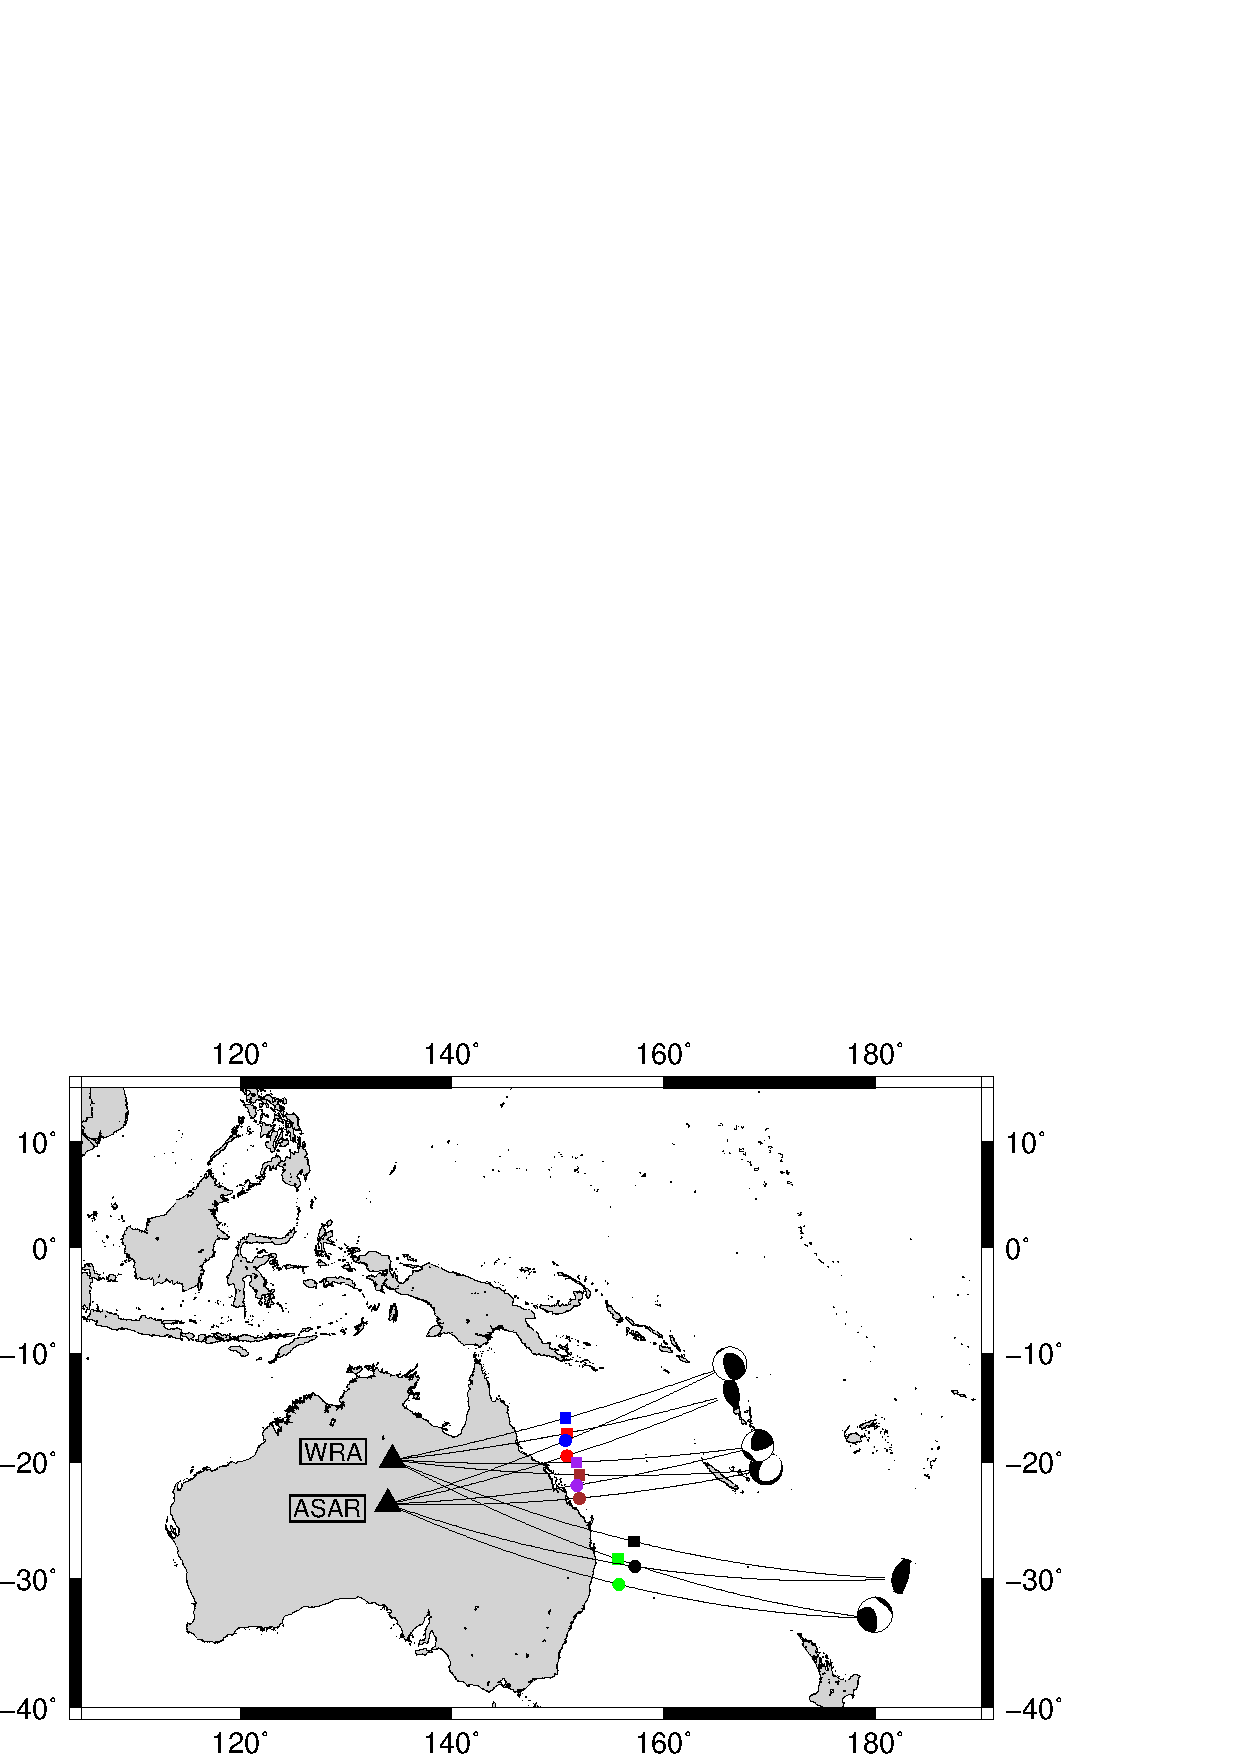
\includegraphics[width=0.8\linewidth]{fig/chap3/evt_au}
\caption{位于澳大利亚中部的WRA和ASAR台阵及表\ref{evt}中第18--23号事件的位置. 黑色三角形表示台阵位置,黑色连线表示地震到台阵的路径. CMB反射点位置用彩色方框和圆圈表示,方框代表WRA,圆圈代表ASAR,每种颜色代表一个地震. }
\label{fig:evt_au}
\end{figure}

前面一节主要分析了CMB界面起伏对PcP、PKiKP/PcP振幅比和PKiKP-PcP走时残差的影响,这一节就CMB上部低
速结构特别是ULVZ结构对观测振幅比和走时残差的影响进行探讨. 结合\citet{McNamara2010}总结的前人对全球范围内超低速带的观测和全球IMS小口径台阵的分布情况,能采样到前人研究所发现的CMB超低速带的只有位于澳大利亚的WRA-ASAR台阵对的数据. 因此,这一节利用对这两个台阵的PcP和PKiKP数据,分析CMB低速或ULVZ结构对PKiKP/PcP振幅比异常的贡献;同时,结合PKiKP-PcP走时残差分析所采样区域的界面起伏变化. 

这里一共选取6个地震事件,其中四个分布在圣克鲁兹群岛至瓦努阿图群岛之间,另外两个位于新西兰的克马德克群
岛. 对于前四个地震,两个台阵到它们的震中距基本在31{\textdegree}--32{\textdegree}之间,PcP反射
点位于CMB上$-$23{\textdegree}S至$-$16{\textdegree}S的位置,8个反射点位置经度变化不大,在CMB
上近似地排成一条线状剖面,并恰好位于\citet{Thorne2004a}利用SKP${}_{diff}$S探测到的ULVZ附近,
并位于\citet{He2012a}所定义的“太平洋异常”西边界上;台阵到其余两个地震的震中距约42{\textdegree}--44{\textdegree},PcP反射点在CMB上$-$30{\textdegree}S附近,在“太平洋异常”西南边界稍稍偏下的
位置. 

\begin{figure}
\centering
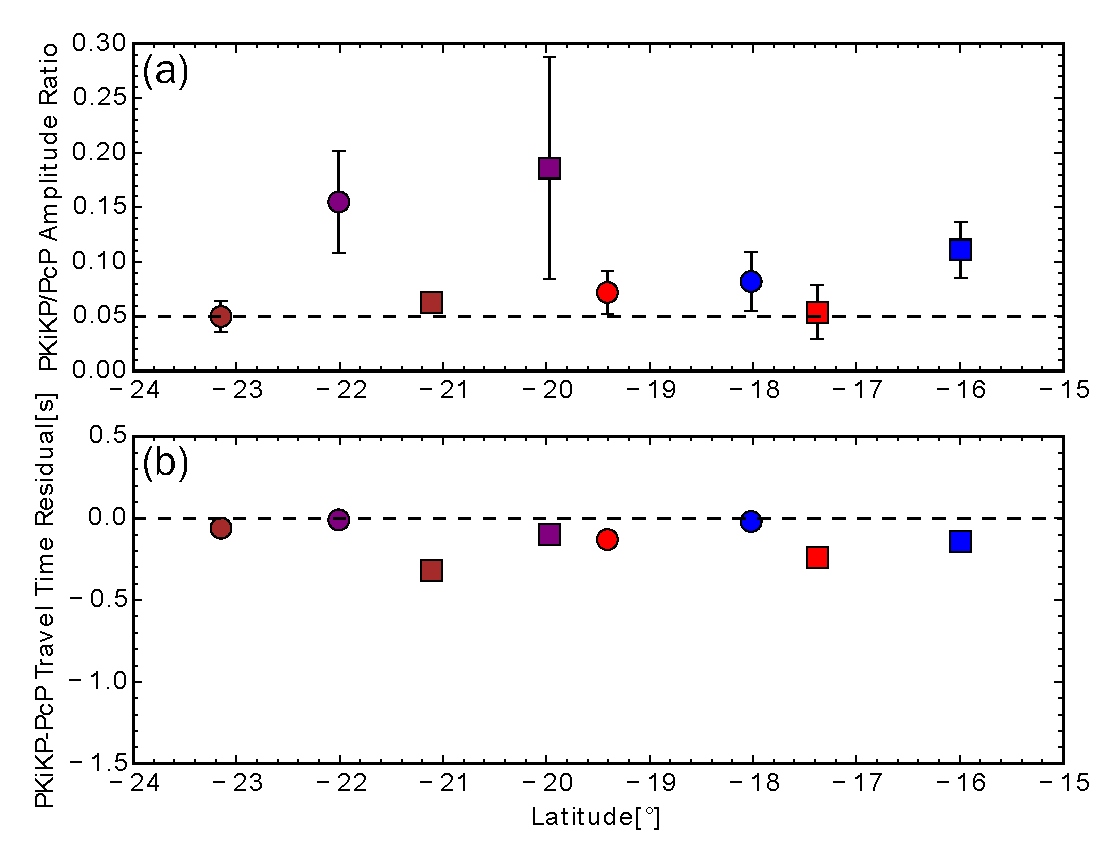
\includegraphics[width=0.7\linewidth]{fig/chap3/au_ratio_tres}
\caption{(a)图\ref{fig:evt_au}中事件-台阵对的PKiKP/PcP振幅比,每个观测点的颜色和形状图\ref{fig:evt_au}中的颜色形状对应. 虚线表示震中距30{\textdegree}时PREM预测的振幅比;(b)每个事件-台阵对的PKiKP-PcP相对PREM的走时残差,颜色表示同(a). 虚线表示走时差于PREM零偏差的位置. }
\label{fig:au_ratio_tres}
\end{figure}

WRA和ASAR仅距离400km,而且每个相邻地震-台阵对的PcP反射点在CMB距离大多在60km左右,有的甚至只有30km,因此比起距离1000km的NVAR和PDAR,这两个台阵更适合探测CMB小尺度的变化. 本研究首先对前四个地震的
数据进行分析,尝试估计CMB变化的横向尺度. 首先看图\ref{fig:evt_au}中连续8个反射CMB反射点的位置,
每个事件相应的反射点相互交错,这样就使得不同事件-台阵对的振幅比和走时残差可以互相参考. 8个事件-台阵对
的平均振幅比显示(图\ref{fig:au_ratio_tres}a),对于同一个地震,WRA和ASAR的平均PKiKP/PcP振
幅比基本上比较接近,这说明两个台阵数据采样到的CMB结构是相似的;褐色和红色表示的反射点对应的振幅比也大
致接近,约为PREM预测值的1.5--2倍左右,而圣克鲁兹群岛事件对应的振幅比均稍稍偏大,但ASAR的振幅比较WRA
的小一些;比较异常的是紫色表示的Vanuatu事件,其振幅比平均值远大于相邻两个CMB采样点的,但可以注意到,平均振幅比的标准差也非常大.由于相邻采样点对应的振幅比并不存在特别大的异常,这里可以推测过大的振幅比并非是CMB或者ICB结构变化造成的. 

与振幅比的局部突然增大相比,走时残差却显得非常稳定,所有的事件-台阵对均显示出微负的走时残差,相邻CMB采样点对应的残差的差别最多不超过0.3秒. 值得注意的是,由ASAR观测到的走时残差都接近零,而对于同一地震,相应的WRA观测总是稍稍偏大约0.1--0.3秒,这表明WRA数据可能存在某种系统性的偏差,比较合理的解释是在WRA台阵侧PKiKP和PcP经历了不同的速度结构,假设这种情况成立,那么由CMB起伏引起的走时残差变化就会更小,因而可以认为采样区域的CMB是比较平坦的,估计的起伏上限也只有数百米,这与之前利用ScP研究CMB起伏的研究结果相似~\citep{Vidale1992a}. 

\begin{figure}[ht]
\centering
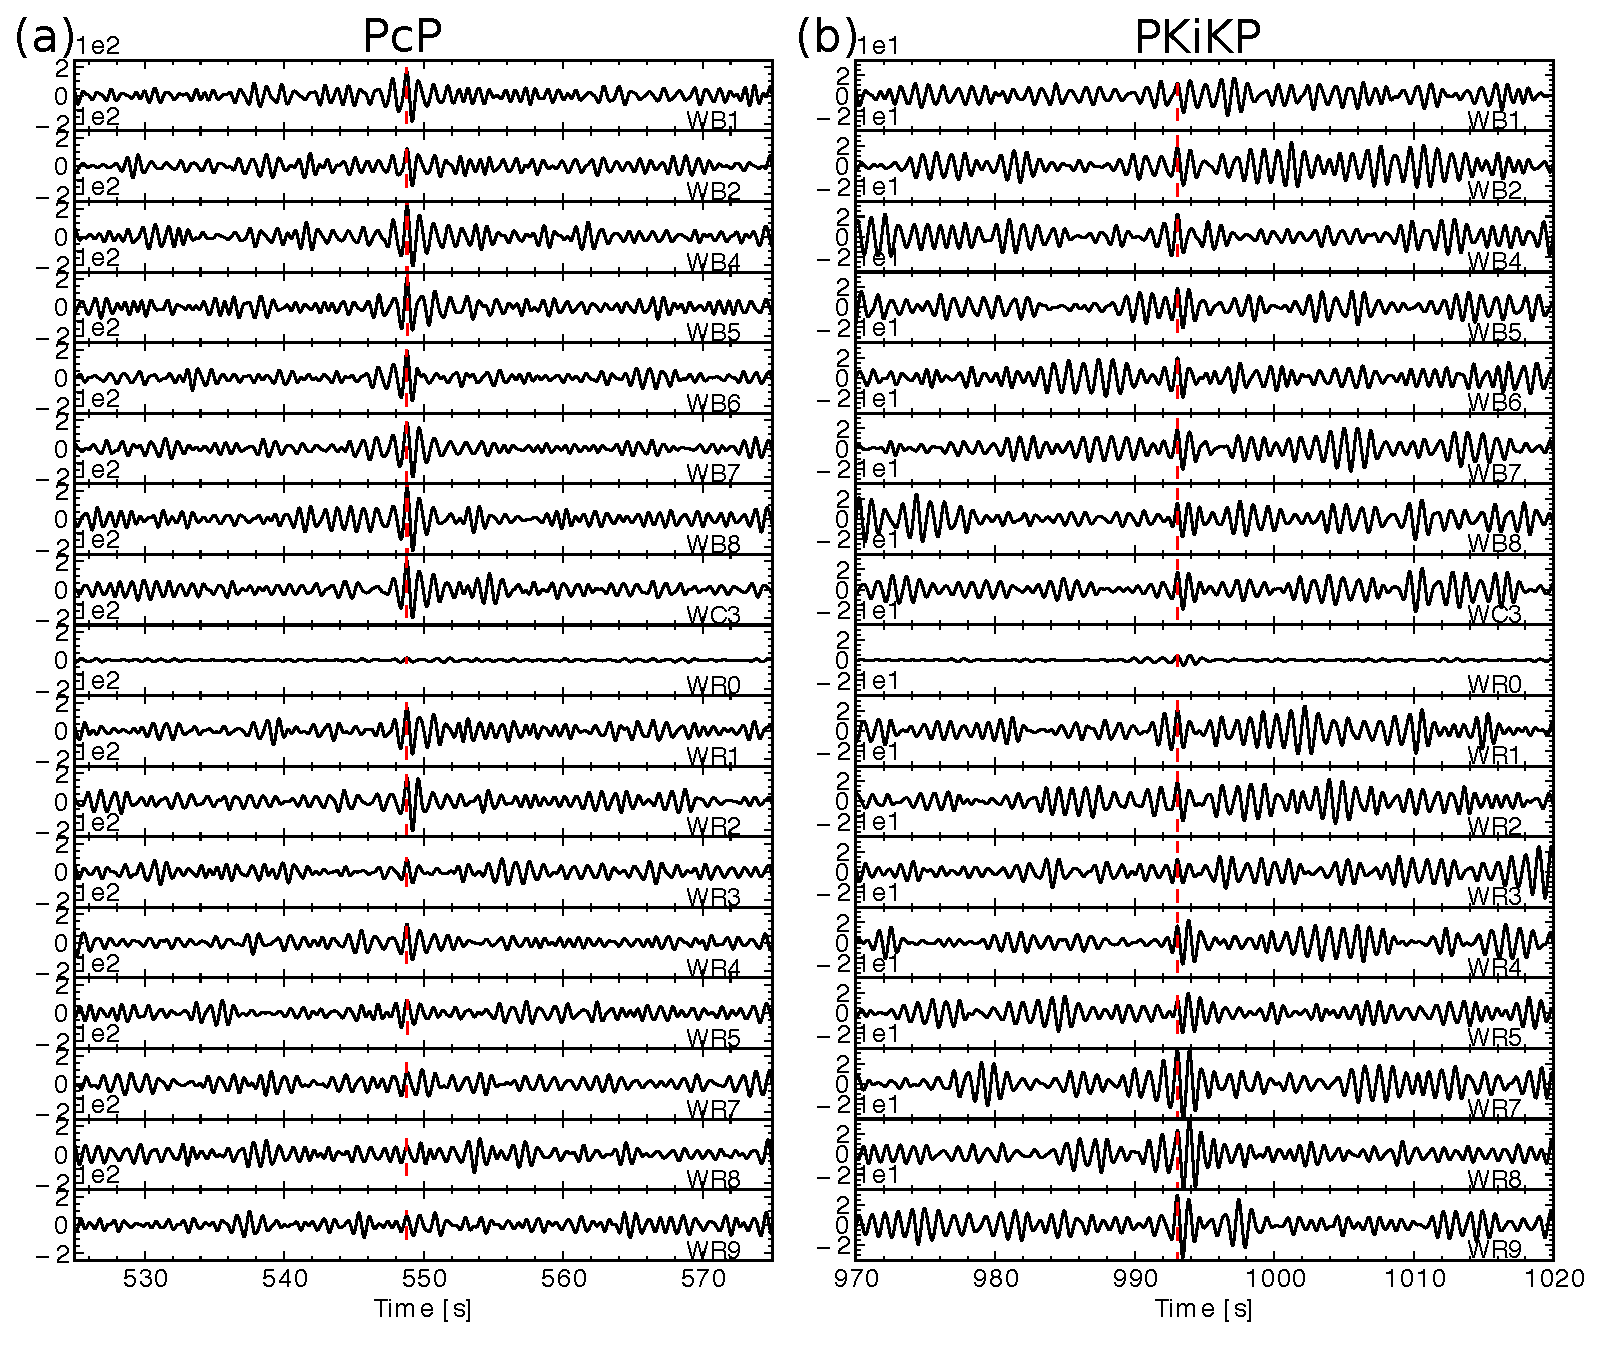
\includegraphics[width=\linewidth]{fig/chap3/pcp_pkikp}
\caption{WRA对表\ref{evt}中第22号地震的PcP(a)和PKiKP(b)记录. 红色虚线标出测量的PcP和PKiKP振幅峰值位置. }
\label{fig:pcp_pkikp}
\end{figure}

再回到PKiKP/PcP振幅比的问题上来. 根据走时残差的结果,推断采样的CMB区域是比较平坦的,那么造成振幅比
突然变化的因素便不会是CMB起伏,可能是由于震源的因素,即在离开震源后,PcP立刻受到较大的衰减,通过比较
震源深度,发现产生振幅比较大的事件震源深度达到200km,可能受到俯冲板块的影响,造成异常的振幅比观测. 虽然台阵记录的不确定性也会造成很大的平均振幅比和标准差,但两个台阵呈现一致的变化,因此可以排除台阵本身的因素. \citet{Koper2004a}在此区域也同样观测到很多异常大的PKiKP/PcP振幅比,但这里并没有发现很多类似的情况,之前研究大振幅比的观测可能是台阵内台站记录存在较大差异的结果,如图\ref{fig:pcp_pkikp}显示的WRA对事件22的PcP和PKiKP记录,所有的台站记录全都按照相同振幅尺度画出,可以发现很多WRX台站记录的PcP振幅要明显偏小,而PKiKP则明显偏大了,这样单道的振幅比就会明显增大. 之前研究通常采用的是所有记录的叠加后的振幅比,即把那些振幅比很大的记录也包含在内了,因此可能得到一个虚假的振幅比异常. 还是以图\ref{fig:pcp_pkikp}的记录为例,如果包含所有WRX台记录,得到的平均台阵振幅比将超过0.25,当舍弃这些小PcP的记录,平均振幅比立刻降到0.1之下(图\ref{fig:au_ratio_tres}a中的褐色方框),且标准差也大大减小了. 通过以上分析,可以认为某些观测到的异常大的振幅比并不是CMB变化所造成的,震源一侧的结构可能对此有很大的贡献,这也可以解释两个台阵振幅比观测的一致性. 除此之外也不能排除过大的振幅比是不正确的震源校正造成的~\citep{Rost2004a},在小震中距情况下,虽然PcP和PKiKP的离源角相差不大,但当它们的出射位置接近辐射花样的节平面的时候,两者的能量可能有显著差异.

%采样区域恰好处于以往研究所定义的超低速带附近,而关于西太平洋低速异常边缘的超低速带研究显示S波波速可以
%达到13\%的降低~\citep{He2006a,He2012a},即使不考虑比较极端的30\%的情况~\citep{Thorne2004a},用ULVZ也足以解释振幅比大于PREM预测一倍左右的观测(图\ref{fig:model_cmb}). 

\begin{figure}[ht]
\centering
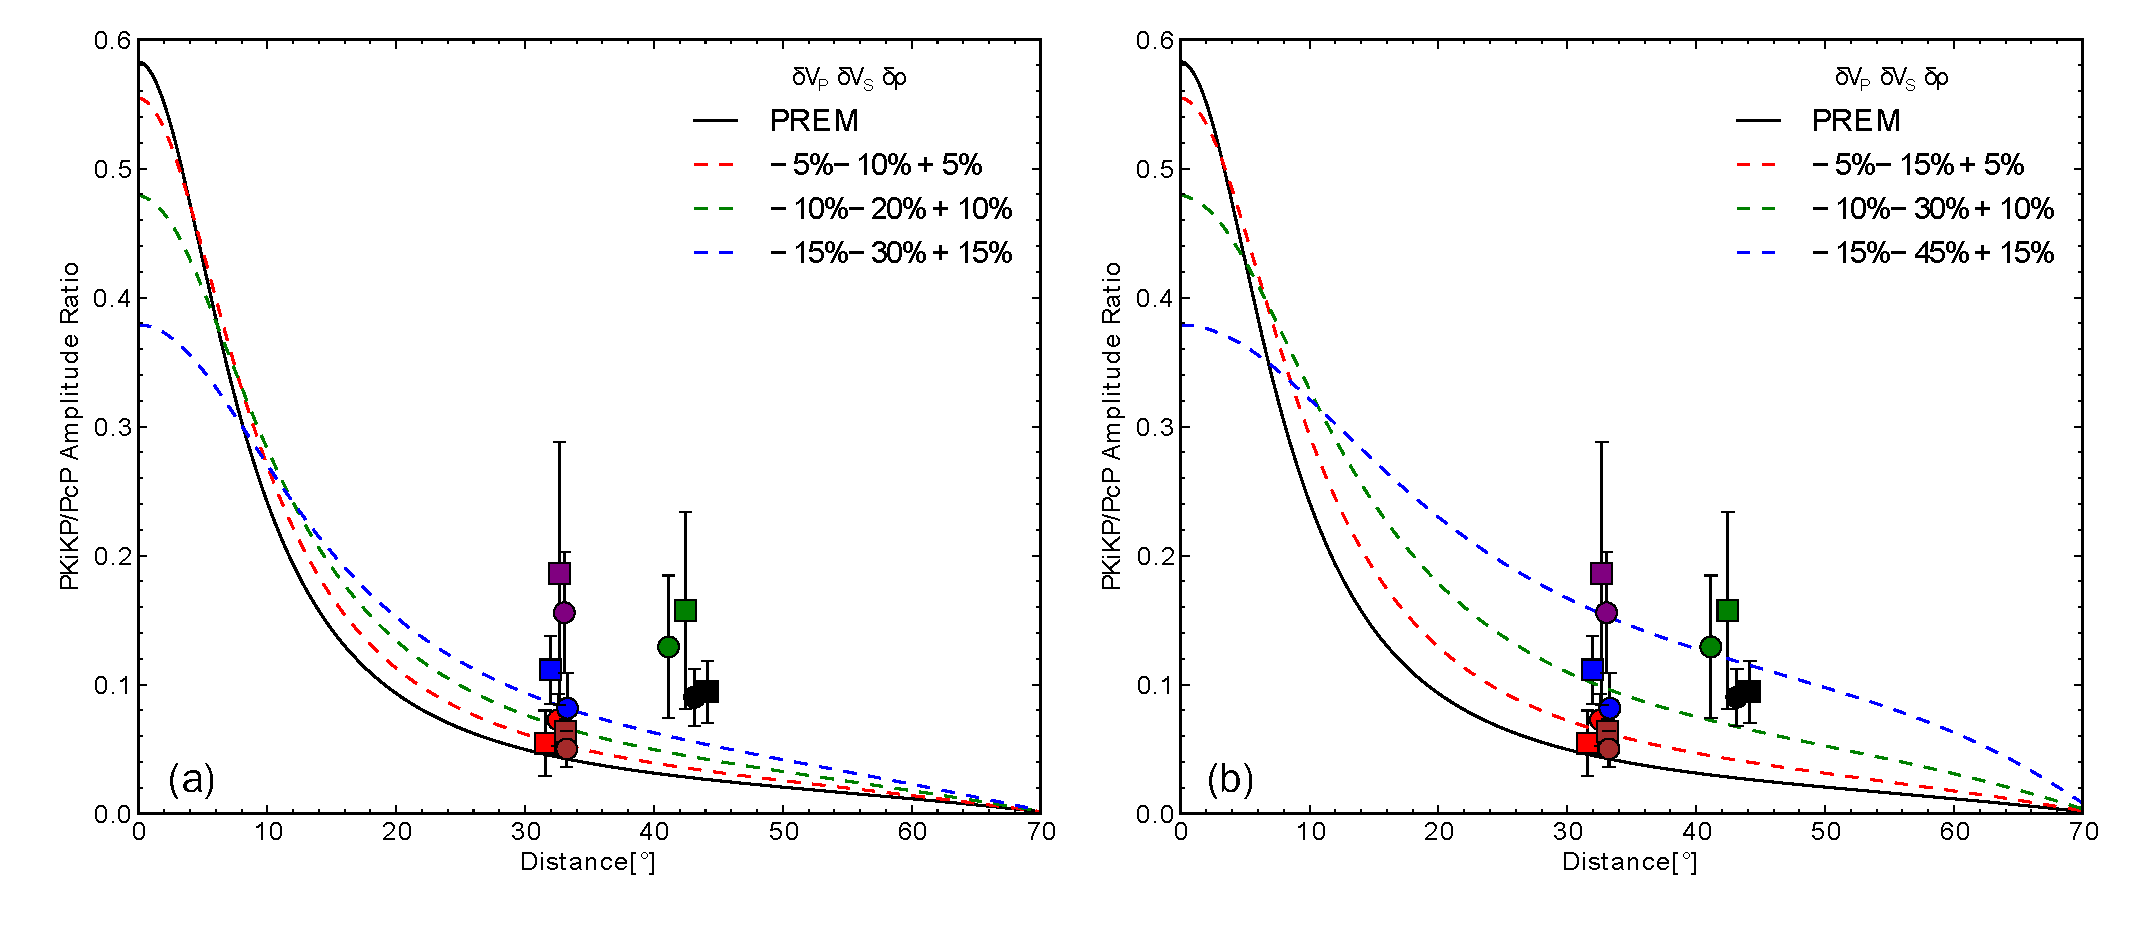
\includegraphics[width=1\linewidth]{fig/chap3/model_cmb}
\caption{不同ULVZ模型参数下的理论PKiKP/PcP振幅比曲线和观测振幅比. (a)$\delta$V${}_P$:$\delta$V${}_S$=1:2,波速的减小和密度的增大以整数倍增加;(b)$\delta$V${}_P$:$\delta$V${}_S$=1:3,参数变化方式同(a). }
\label{fig:model_cmb}
\end{figure}

由于采样区域恰位于前人定义的ULVZ附近,关于西太平洋CMB低速异常边缘的研究显示CMB底部S波波速可以降低13\%~\citep{He2006a,He2012a},假设实际的ICB物理参数与PREM描述一致,则本文观测到的振幅比中的较小值可以和之前的研究结果相吻合(图\ref{fig:model_cmb}),除了异常的大振幅比,图8中稍大的振幅比可能需要用20\%至30\%的S波波速降低来解释. 对于位于“太平洋异常”西南边界之外的两个采样点对应的振幅比,可能还需要用更大的S波波速降低来解释(大于30\%). 考虑到观测的不确定性,仅用PKiKP/PcP振幅比仍然不能很好地约束CMB参数,这里的结果也仅能为之前的研究提供一些支持,同时也体现出用振幅比研究界面参数的局限性. 还可以注意到,采样“太平洋异常”西边界的PcP波形与PKiKP相似,主反射震相之前并没有出现明显的信号,这说明即使超低速层是存在的,这一层的顶部也并非是一个不连续界面,或者层的厚度很薄,小于PcP的波长(约13km),不足以产生可观测到的反射波,这也与之前利用ScP的研究该区域ULVZ厚度的结果相吻合~\citep{Rost2010a}.
